\singlespacing
\chapter{Diseño, construcción y aplicación de un microespectrómetro}
\label{chap:microsp}
\spacing{1.5}

\hspace{0.5cm}En el Capítulo \ref{chap:zeiss} se realizó una descripción cuantitativa de los defectos: se determinó su área, su diámetro equivalente, la cantidad de defectos presentes en cada banda, etc. Dicho análisis permitió entender las especificaciones técnicas de \textit{scratch \& dig} y de la ISO 10110, lo que resulta fundamental para establecer las bases de futuros acuerdos con los fabricantes de los componentes ópticos. Al mismo tiempo, los resultados de la población de defectos en general [\ref{sec:defpob}] detectados con el algoritmo permitieron establecer los criterios de diseño óptico del microespectrómetro que se explica en el presente capítulo.

Como se explicó en el Capítulo \ref{chap:introd}, un microespectrómetro es un instrumento de medición híbrido que integra la capacidad de magnificación y de resolución ópticas de un microscopio con la capacidad de inferir las propiedades ópticas de un material de un espectrómetro. En este capítulo se describe el diseño y la construcción de un microespectrómetro que permitió realizar una caracterización de las propiedades ópticas del filtro y de sus defectos a través de los espectros de transmisión [\ref{sec:montcontmsp}]. En la Sección \ref{sec:prot0} muestran las características del primer prototipo desarrollado con equipamiento disponible en el laboratorio. Dicho prototipo en conjunto con los resultados y análisis del Capítulo \ref{chap:zeiss} permitieron establecer los criterios de elección de la fuente de luz y del espectrómetro [\ref{sec:fteluzyesp}], determinar la longitud del recorrido y la precisión mínima necesaria de la platina que se desarrolló [\ref{sec:platina}] y la resolución óptica necesaria del microscopio desarrollado para caracterizar los defectos de diámetro mayores a 20$\mu m$ de diámetro [\ref{sec:disop}]. Luego se explica el proceso de montaje y alineación preliminar del microespectrómetro [\ref{sec:montalin}] así como su puesta en foco y la determinación de la resolución espacial [\ref{sec:focoresol}]. Posteriormente se explica la integración de una cámara web al microespectrómetro lo que permitió la adquisición simultánea de imágenes digitales y de espectros de transmisión y cuya área de adquisición fue elegida con un \textit{joystick} y visualizada en vivo a través de una interfaz gráfica [\ref{sec:camwebgui}].

Asimismo, se muestran los resultados de los espectros de transmisión de cada banda del filtro y su comparación con la hoja de datos reportada por el fabricante [\ref{sec:espectransm}]. Finalmente, se muestran los resultados de la caracterización espectral de los defectos denominados manchas ó defectos de transmisión [\ref{sec:defctma}] y de los agujeros ó huecos [\ref{sec:defctag}].

%%%%%%%%%%%%%%%%%%%%%%%%%%%%%%%%%%%%%%%%%%%%%%%%%%%%%%%%%%%%%%%%%%%%%%%%%%%%%%%%%%%%%%%%%%%%%%%%%%%%%%%%%%%%%%%%%%%%%%%%%%%%%%%%%%%%%%%%%%%%%%%%%%%%%%%%%%%%%%%%%%%%%%%%%%%%%%%%%%%%%%%%%%%%%%%%%%%%%%%%%%%%%%%%%%%%%%%%%%%%

\singlespacing
\section{Prototipo preliminar\href{https://github.com/jrr1984/Prototipo0\_S-D\_SpectralGUI/blob/master/barrido/std/main.py}{\faGithub}}
\label{sec:prot0}
\spacing{1.5}

\hspace{0.5cm}El desarrollo del prototipo preliminar que se muestra en esta sección permitió por un lado establecer los criterios de elección de la fuente de luz y del recorrido y la precisión necesarias de la platina desarrollada para poder adquirir el espectro e imágenes del filtro completo. Como buena práctica de prototipado de instrumentos de medición se utilizaron componentes y equipamiento disponibles en el laboratorio, es decir que no se incurrió en gastos adicionales de dinero a excepción del costo del material de las impresiones 3D del soporte del filtro. Por otro lado, a partir del desarrollo del software automatizado de adquisición y de visualización de los resultados de este prototipo se establecieron las características deseadas y esperadas del prototipo final desarrollado. De esta manera, el prototipo permitió establecer la factibilidad del desarrollo del equipo.

Como objetivo general se propuso desarrollar un sistema integral de caracterización de filtros ópticos de interferencia utilizados en cámaras hiper y multiespectrales. Inicialmente se propusieron tres objetivos específicos:
\begin{enumerate}
\item Desarrollar un sistema automatizado de adquisición del espectro de transmisión de cada una de las bandas del filtro.$\xrightarrow{}$ \href{https://github.com/jrr1984/Prototipo0\_S-D\_SpectralGUI/blob/master/barrido/std}{\faGithub}

\item Determinar un mapa hiperespectral ($\textit{x}$,$\textit{y}$,$\lambda$) del filtro.$\xrightarrow{}$ \href{https://github.com/jrr1984/Prototipo0\_S-D\_SpectralGUI/blob/master/spectral\_gui/main.py}{\faGithub}

\item Integrar un sistema de detección y caracterización de los defectos del filtro.
\end{enumerate}

A continuación se describen los primeros dos objetivos que fueron abarcados por el prototipo preliminar descripto en esta sección. Respecto del primer objetivo, se montó el arreglo experimental que se muestra en las Figuras \ref{fig:setup0}, \ref{fig:setup01} y \ref{fig:setup02}. 

\begin{figure}[H]
	\centering
	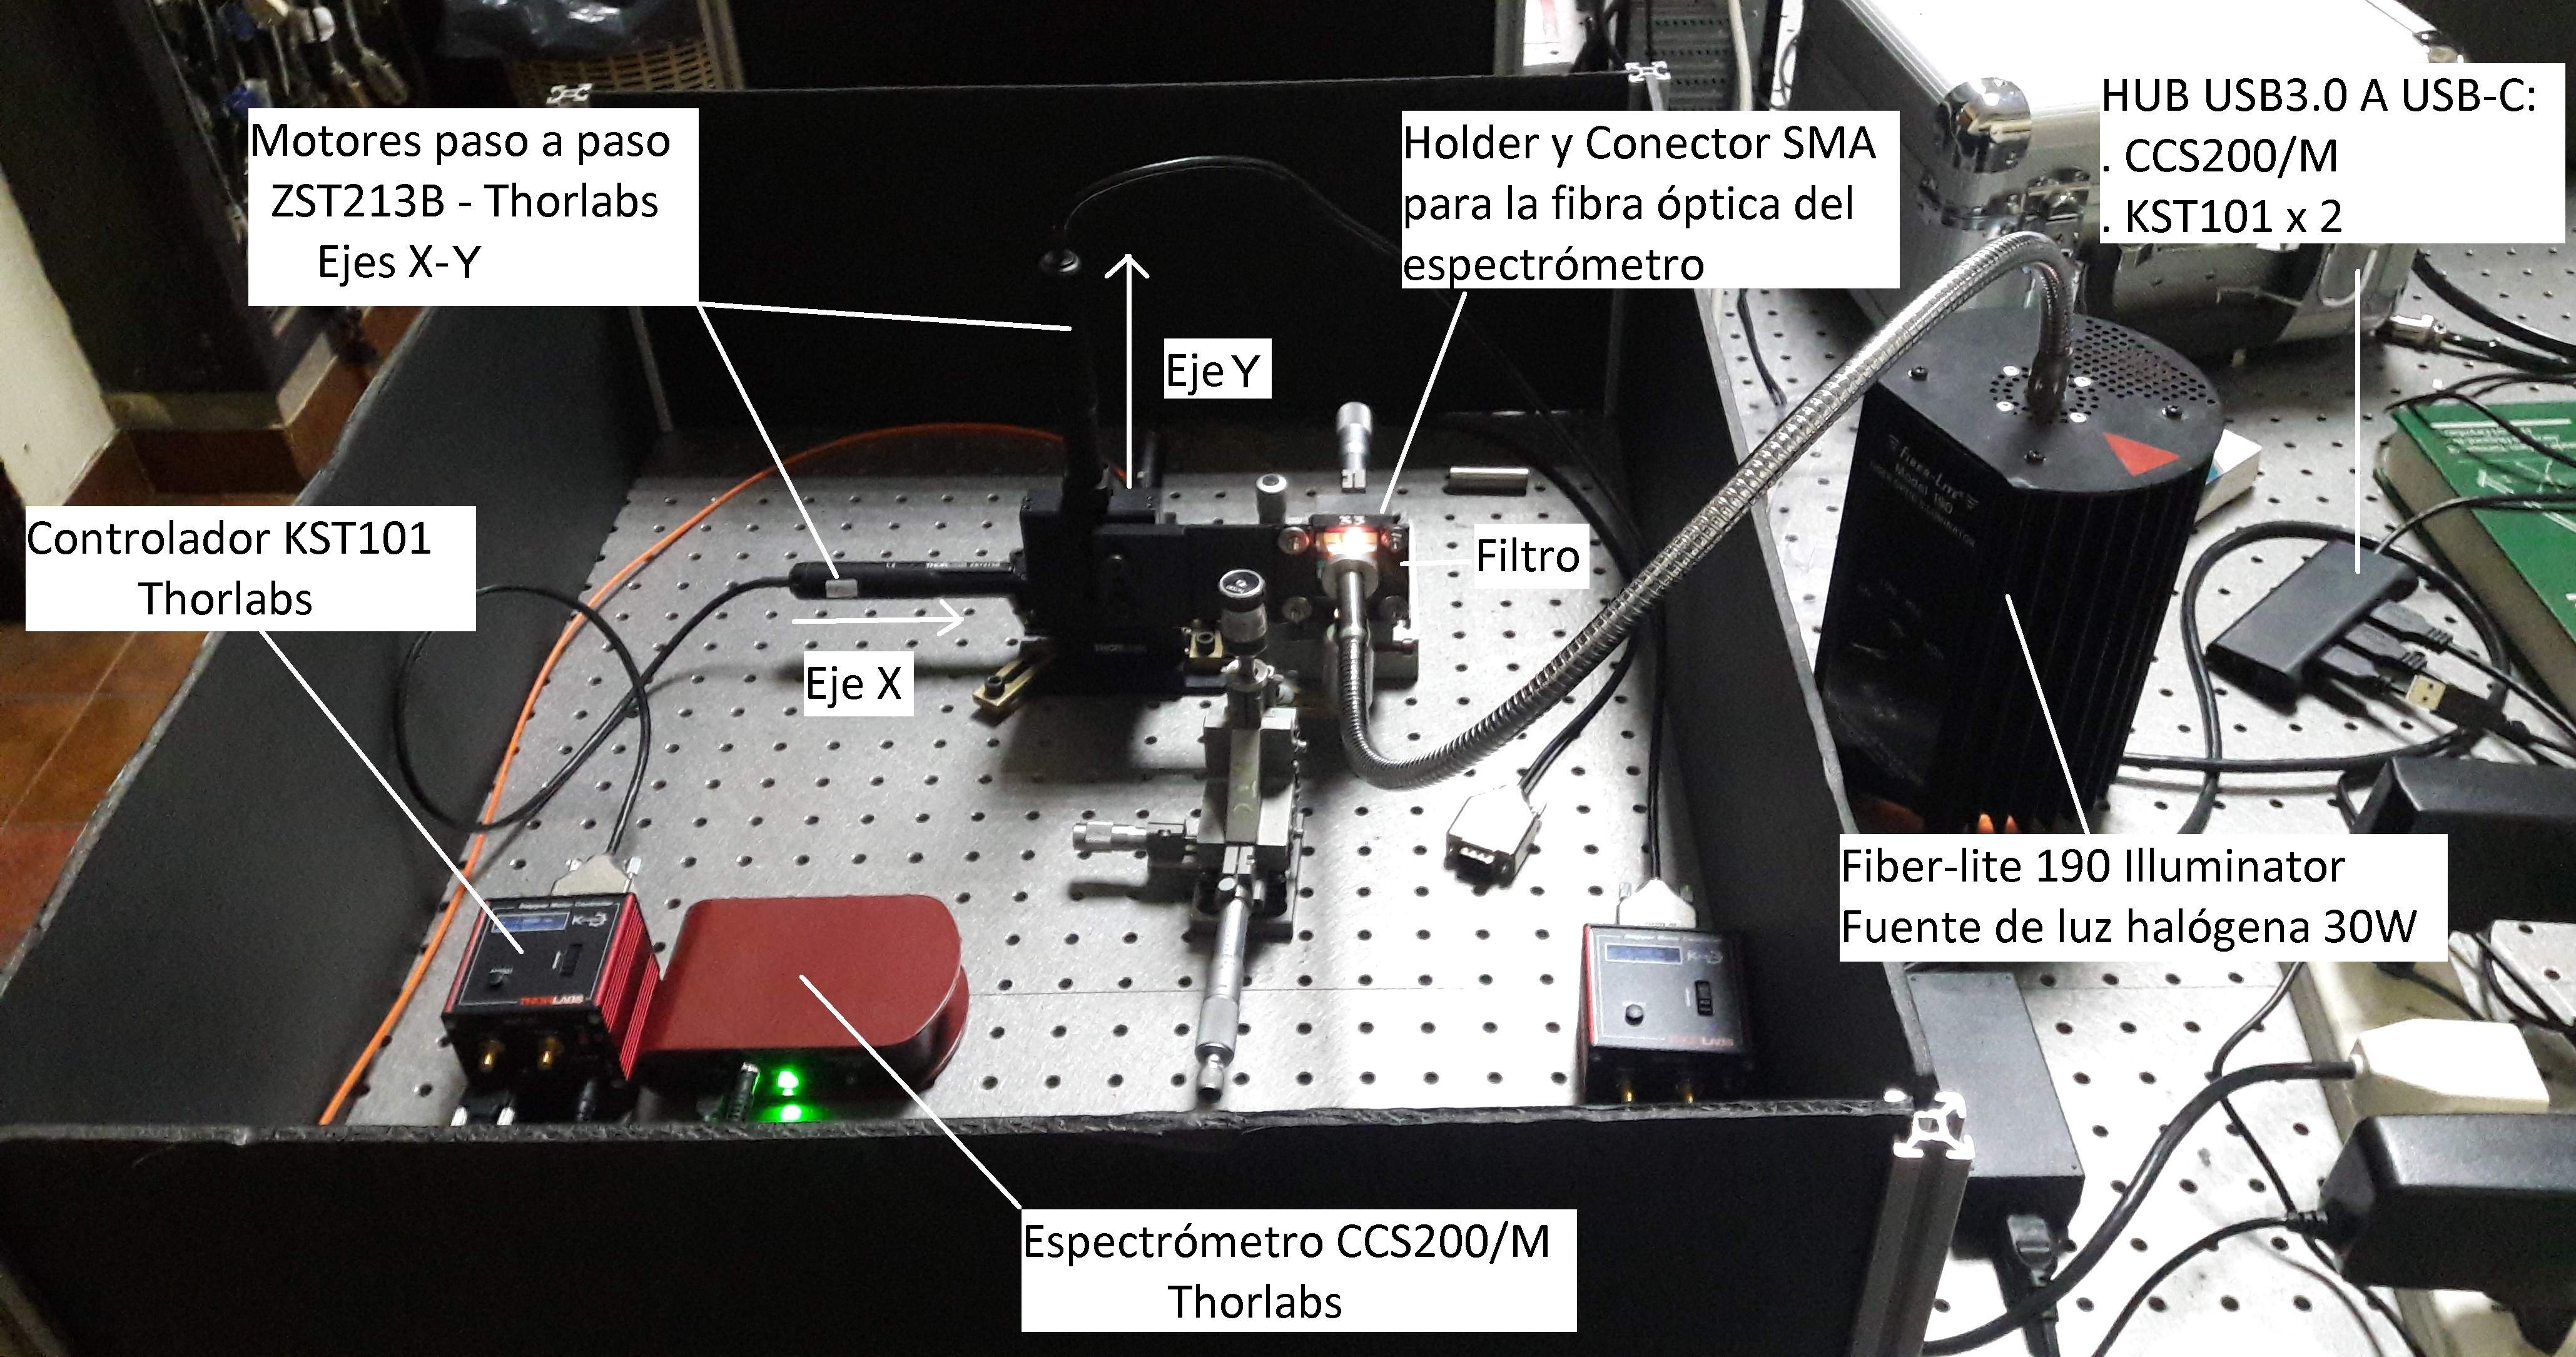
\includegraphics[width=1.0\textwidth]{Figs/microespectrometro/setupbarridooriginal.jpg}
	\caption{Arreglo experimental del prototipo preliminar.}
	\label{fig:setup0}
\end{figure}

\begin{figure}[H]
	\begin{floatrow}
		\ffigbox{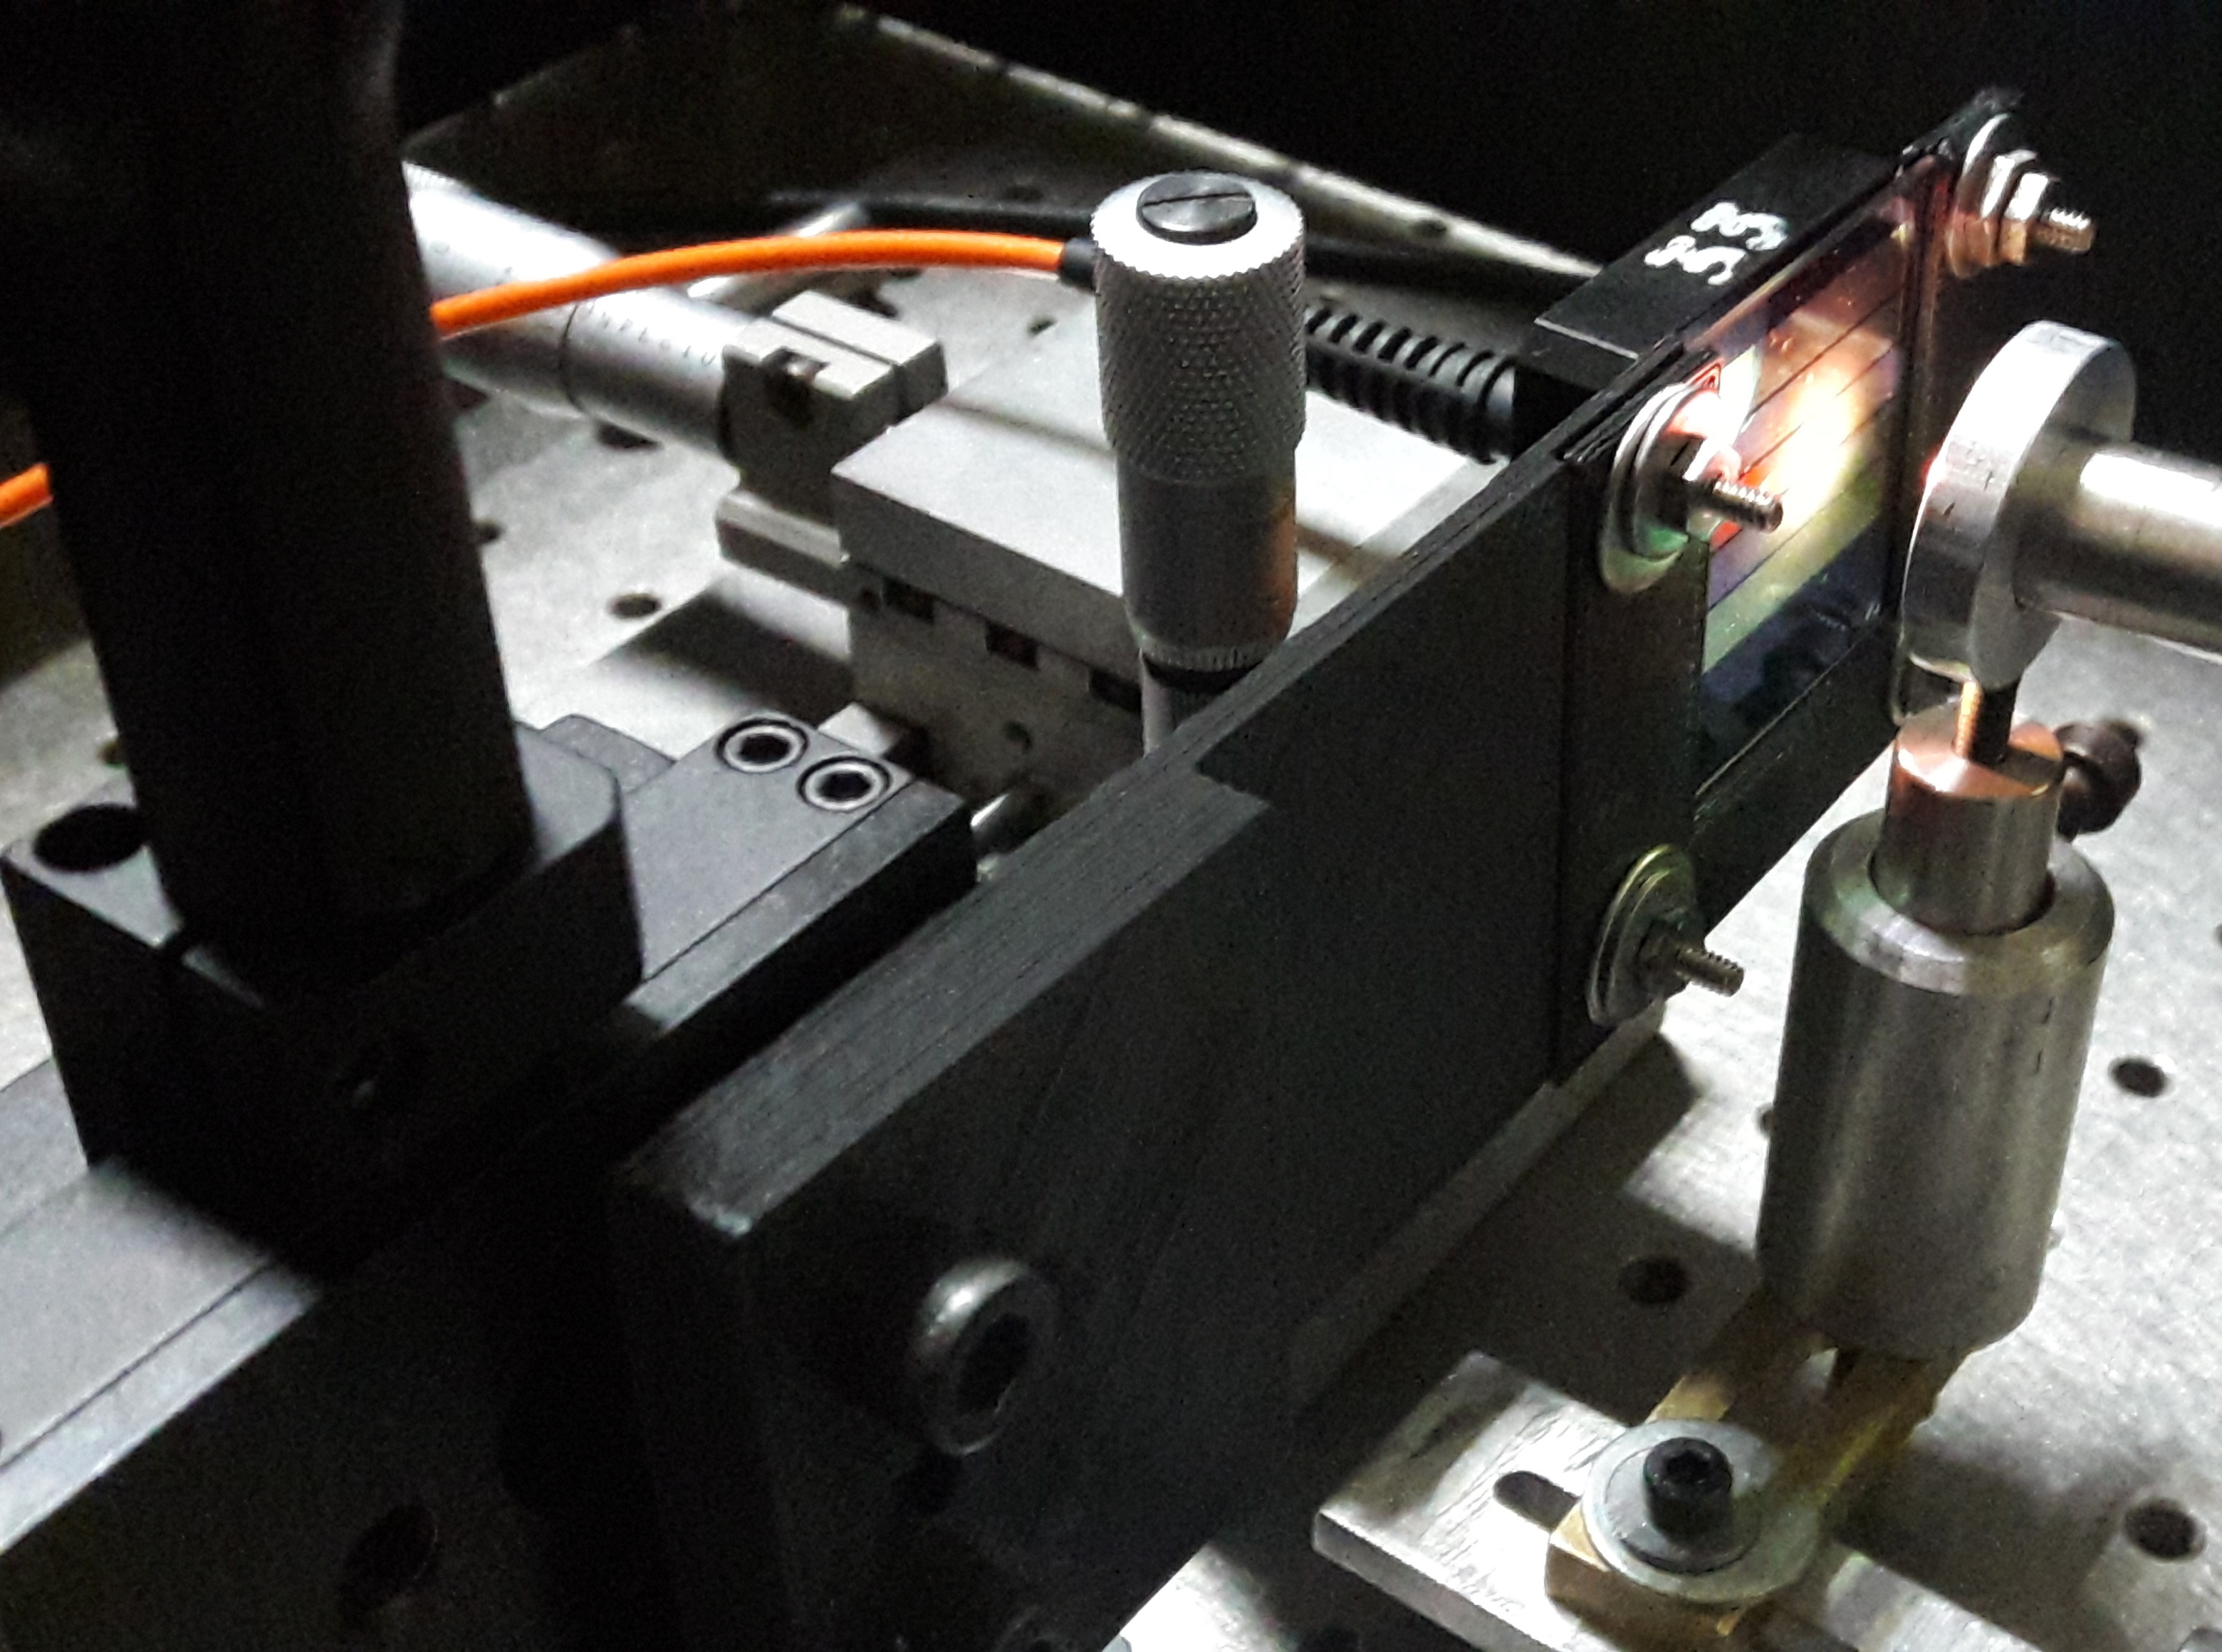
\includegraphics[scale=0.073]{Figs/microespectrometro/montajesetup0.jpg}}{\caption{Vista lateral del montaje del filtro sobre el soporte que se encuentra atornillado con unos tornillos M6 a la plataforma motorizada de Thorlabs.}\label{fig:setup01}}
		\ffigbox{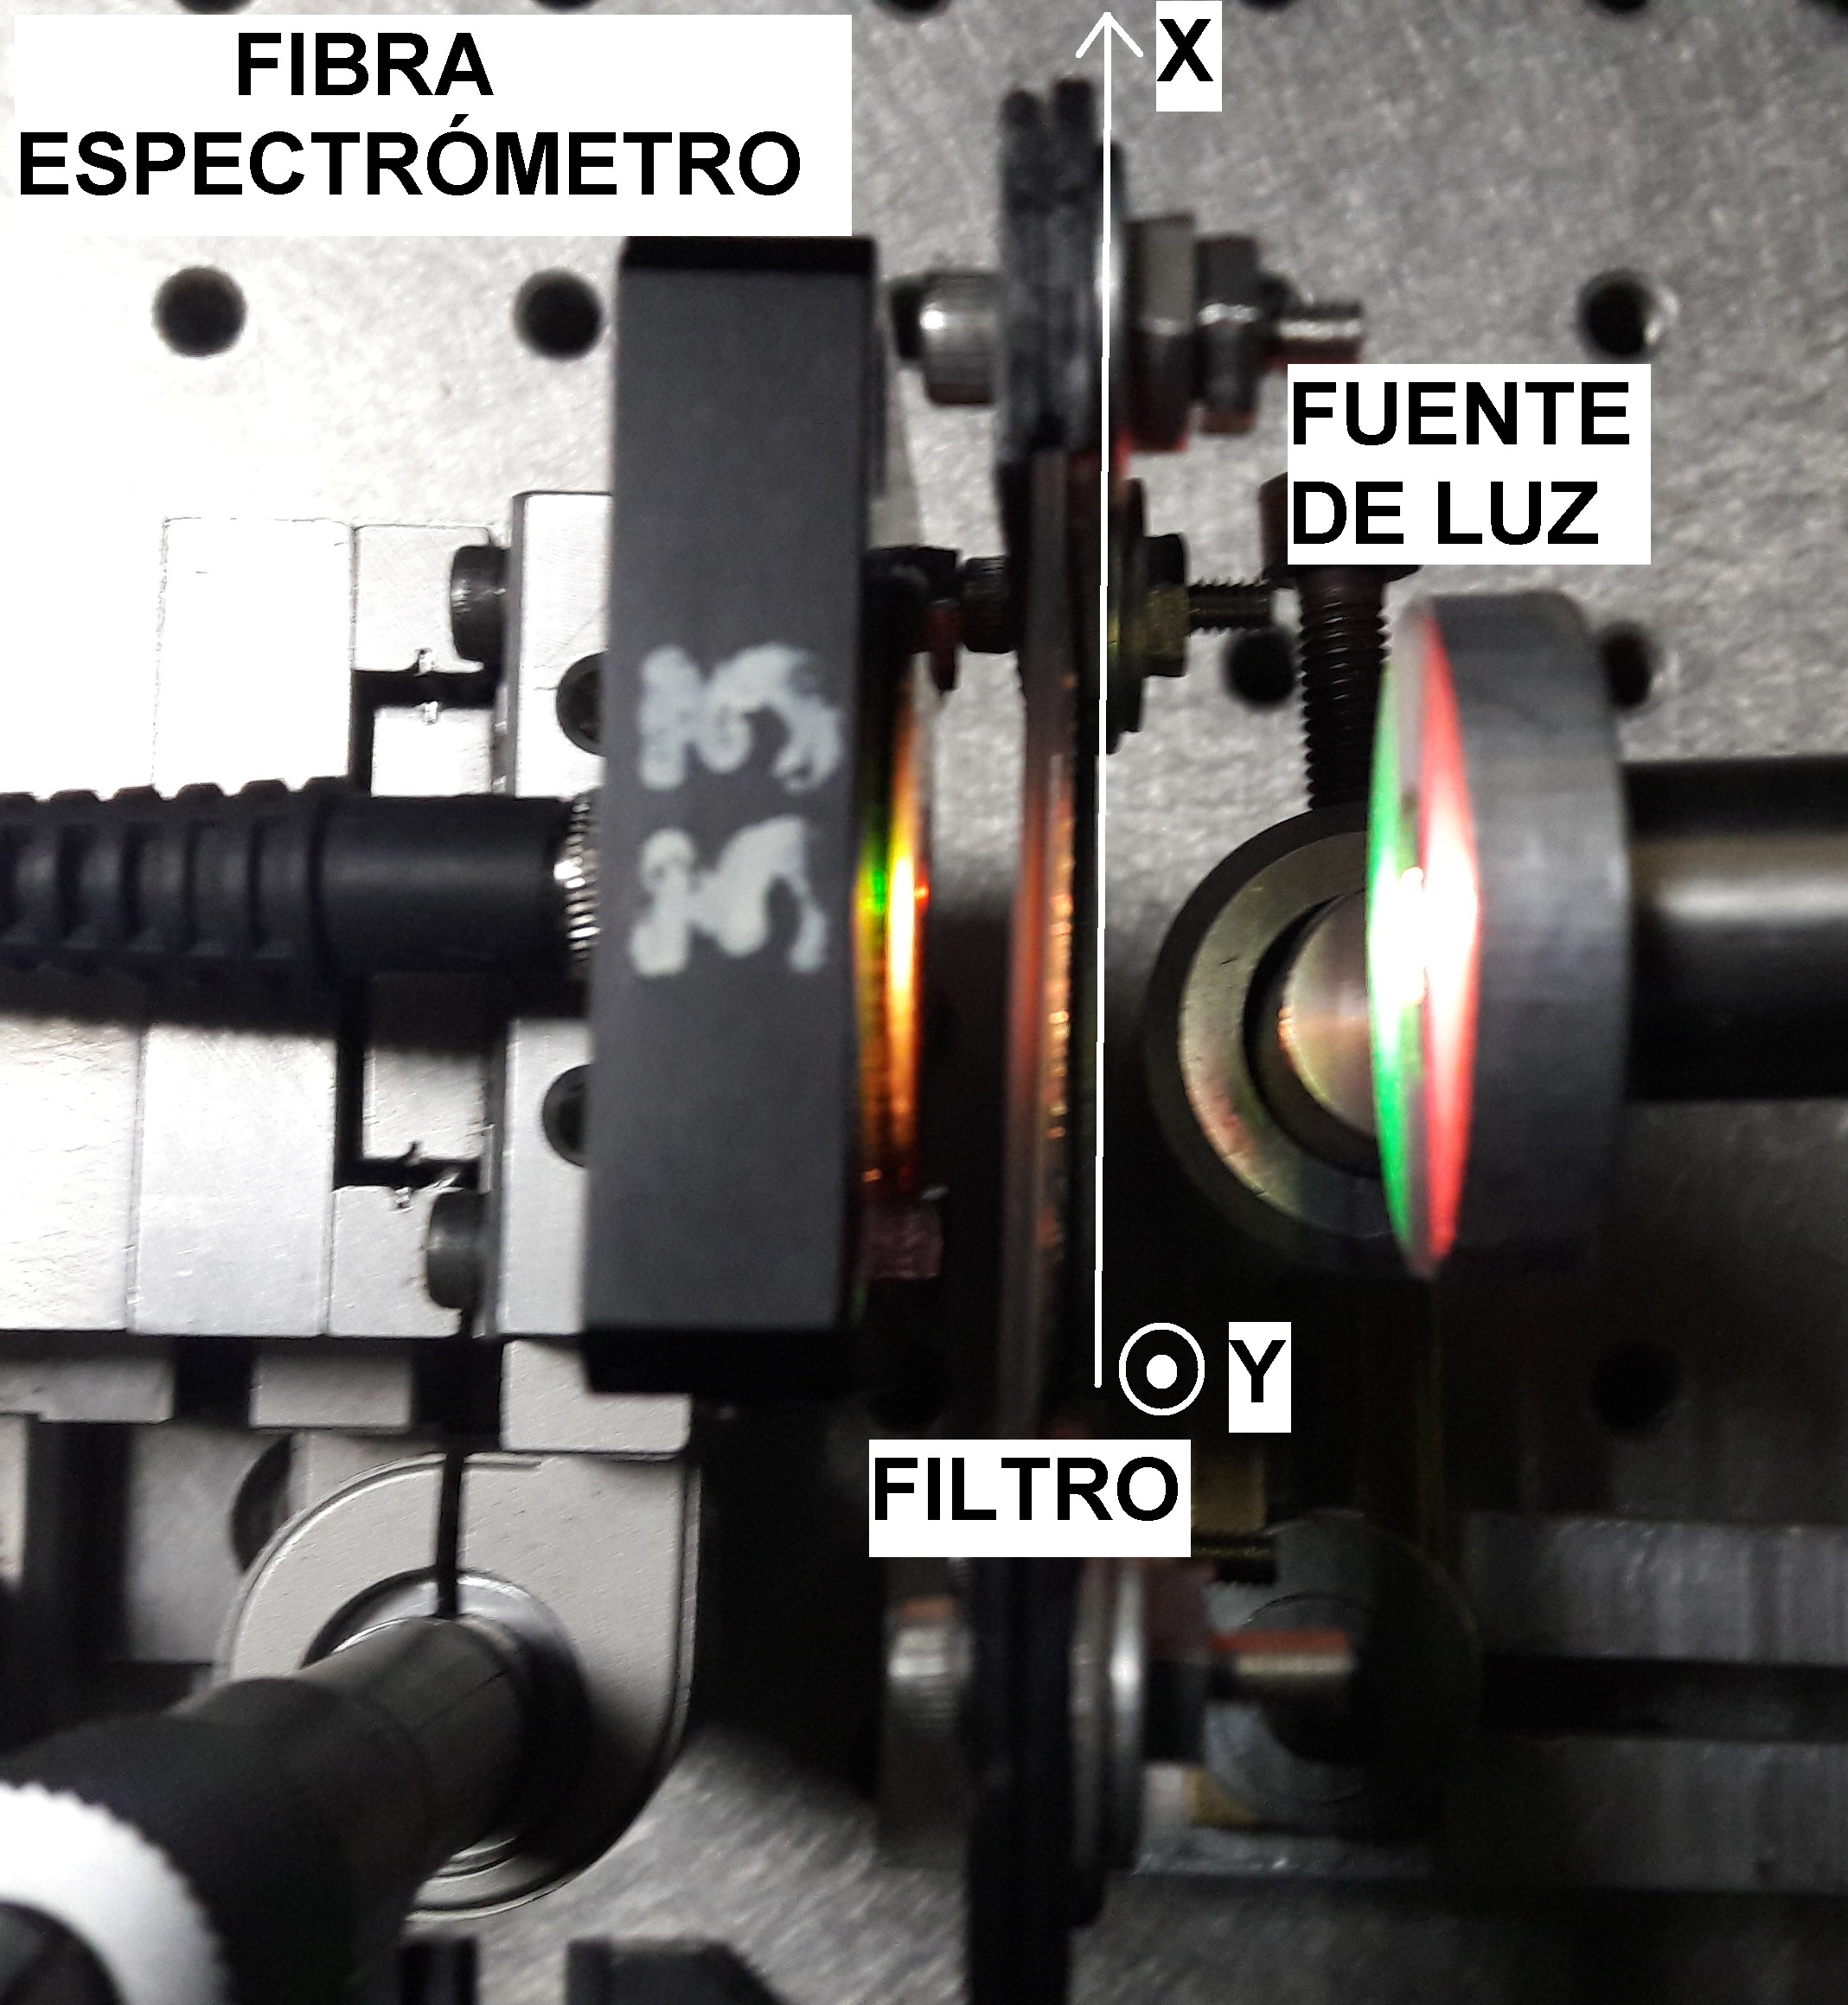
\includegraphics[scale=0.073]{Figs/microespectrometro/5.jpg}}{\caption{El filtro se mueve en los ejes $\textit{x}$ e $\textit{y}$. La fuente de luz y la fibra del espectrómetro se encuentran inmóviles. }\label{fig:setup02}}
	\end{floatrow}
\end{figure}

Con una fuente de luz halógena, modelo \href{https://dolan-jenner.com/products/fiber-lite-190}{\textit{Fiber-lite 190 Illuminator}}, se incidió perpendicularmente sobre el filtro y su transmisión fue detectada por la fibra óptica de un espectrómetro modelo \href{https://www.thorlabs.com/thorproduct.cfm?partnumber=CCS200/M#ad-image-0}{CCS 200/M} de la empresa Thorlabs (\textit{Driver} de \textit{python}: \href{https://github.com/jrr1984/Prototipo0\_S-D\_SpectralGUI/blob/master/syst/CCS200.py}{\faGithub}). De la misma manera en que se realizó el \textit{Tile Scan} del filtro completo con el microscopio Zeiss explicado en la sección \ref{subs:tilsc} (Ver Figura \ref{fig:tilescan}), se desplazó el filtro a lo largo del eje x, barriendo en `filas' y realizando el desplazamiento vertical en los extremos del máximo recorrido de los tornillos accionados por los motores paso a paso que fue de 13 mm. Dicho desplazamiento fue realizado con una plataforma de tres grados de libertad, modelo \href{https://www.thorlabs.com/thorproduct.cfm?partnumber=MT3/M}{MT3/M} de la empresa Thorlabs, cuyos tornillos micrométricos fueron intercambiados por unos motores paso a paso modelo \href{https://www.thorlabs.com/thorproduct.cfm?partnumber=ZST213B}{ZST213B} cuyos controladores fueron también de la empresa Thorlabs, modelo \href{https://www.thorlabs.com/thorproduct.cfm?partnumber=KST101}{KST101} (\textit{Driver} de \textit{python}: \href{https://github.com/jrr1984/Prototipo0\_S-D\_SpectralGUI/blob/master/barrido/std/thor\_stepm.py}{\faGithub}). Como las dimensiones de la región comprendida por las cinco bandas del filtro es de 27 mm x 25 mm, con esta plataforma no se pudo realizar una adquisición del filtro completa en una sola configuración como la propuesta. El \textit{software} automatizado de adquisición del espectro de transmisión del filtro desarrollado para este prototipo [\href{https://github.com/jrr1984/Prototipo0\_S-D\_SpectralGUI/tree/master/barrido/std}{\faGithub}] fue expandido en el prototipo final y se lo explica en la Sección \ref{sec:softadq}.


No se utilizó ningún arreglo óptico ni para enfocar la fuente de luz en el filtro ni para enfocar su transmisión divergente sobre la fibra óptica del espectrómetro. No se caracterizó la resolución óptica con la que se realizaron las mediciones con el espectrómetro en este prototipo ni el tamaño del objeto medido sobre la superficie del filtro. La resolución óptica y magnificación necesarias para medir los defectos del filtro fueron establecidas a partir de los resultados del Capítulo \ref{chap:zeiss} y fueron consideradas en el diseño óptico del microespectrómetro desarrollado que se explica en la Sección \ref{sec:disop}.


Respecto del segundo objetivo específico propuesto relacionado con la determinación de un mapa hiperespectral ($\textit{x}$,$\textit{y}$,$\lambda$) del filtro, se adquirió el espectro de transmisión de una región del filtro con dimensiones iguales 13 mm en el eje $\textit{x}$ y de 24.6 mm a lo largo del eje $\textit{y}$ (las cinco bandas junto al cromo que las separa tienen una altura de 25 mm, ver Figura \ref{fig:dimsfiltr}). El área del filtro adquirida fue el resultado de unir las mediciones de dos barridos cuyas dimensiones fueron para cada uno, de 13 mm a lo largo del eje $\textit{x}$ y de 12.2 mm a lo largo del eje $\textit{y}$. Los ejes fueron definidos de acuerdo al sistema de coordenadas de la Figura \ref{fig:setup02} y el paso del desplazamiento de los motores de cada eje fue de 50 $\mu m$. La adquisición fue realizada en dos etapas debido a la limitación del recorrido de los tornillos desplazados por los motores paso a paso como se explicó anteriormente. De esta manera se adquirió en primer lugar la región superior del filtro que contiene a las bandas azul, verde y parte de la pancromática con una cierta altura de la fuente de luz y de la fibra del espectrómetro. La fuente y la fibra se encontraban montadas sobre unos posicionadores micrométricos con los cuales se varió su altura respecto del filtro para poder medir la región inferior del filtro que contenía la región faltante de la banda pancromática, la banda roja y la banda del NIR. La fuente de luz y la fibra del espectrómetro fueron posicionadas lo más cerca posible del filtro, sin intervenir su libre desplazamiento para realizar el barrido, con el fin de minimizar el tiempo de integración de cada medición del espectro de transmisión que fue de 1 ms.

Con el objetivo de visualizar una imagen completa del filtro como la que se obtuvo con el microscopio Zeiss (Ver Figura \ref{fig:supfiltrocondensador}) pero que contenga además la información espectral de cada medición se desarrolló una interfaz gráfica interactiva que se muestra en la Figura \ref{fig:GUI00}.

\begin{figure}[H]
	\centering
	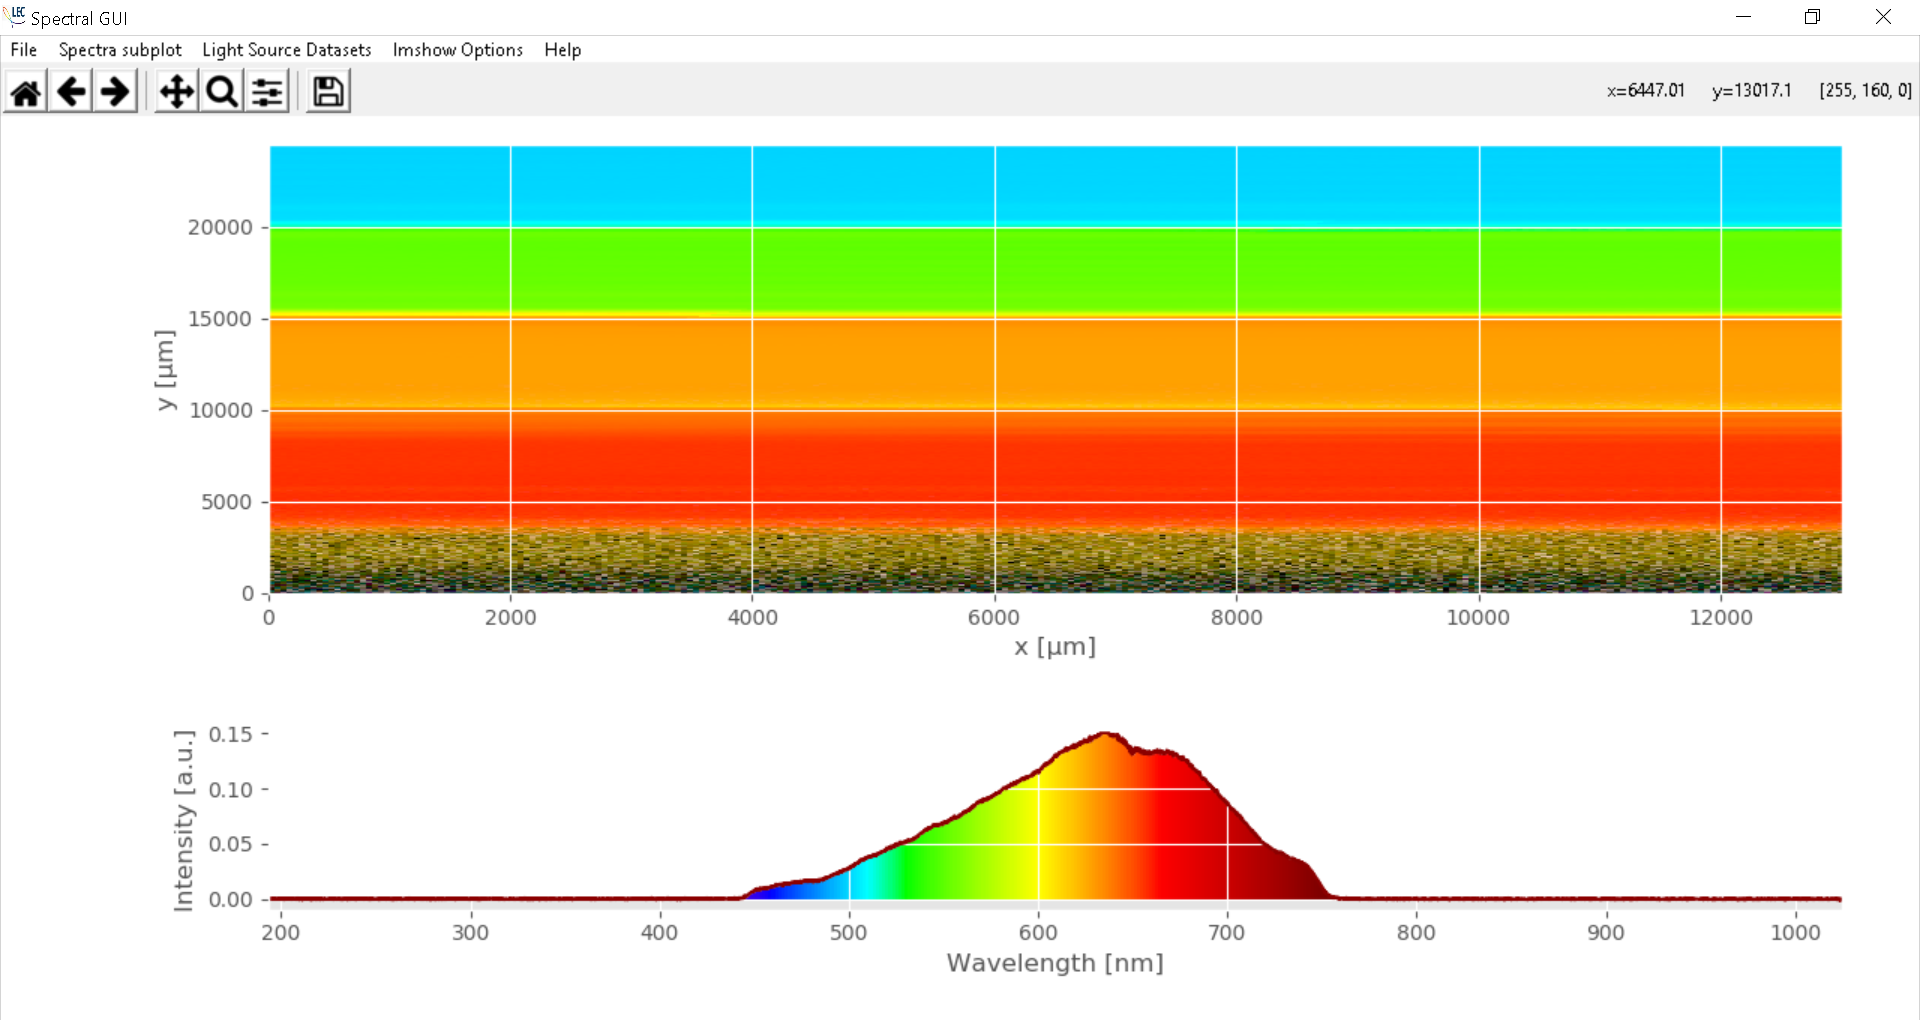
\includegraphics[width=1.0\textwidth]{Figs/microespectrometro/guirgb.png}
	\caption{Interfaz gráfica con el \textit{imshow} en RGB.}
	\label{fig:GUI00}
\end{figure}


La interfaz gráfica fue realizada [\href{https://github.com/jrr1984/Prototipo0\_S-D\_SpectralGUI/blob/master/spectral\_gui/main.py}{\faGithub}] con la librería	 \href{https://wiki.python.org/moin/TkInter}{\textit{Tkinter}}. El barrido completo que se muestra en la imagen del mapa de colores de la Figura \ref{fig:GUI00} estuvo compuesto por 127920 mediciones de espectros de transmisión, que tomaron aproximadamente 18 horas de medición en total (Control remoto de la computadora con \href{https://anydesk.com/es}{AnyDesk} y control del experimento vía \href{https://pypi.org/project/cutelog/}{cutelog}, ver Sección \ref{sec:softadq}). Con la librería \href{https://pypi.org/project/colorpy/}{ColorPy} se obtuvo una tupla RGB a partir del espectro medido y cada tupla fue asignada a una cierta posición del filtro. El conjunto total de todas las posiciones del filtro medidas estuvo formado por una matriz de 492 filas y 260 columnas. Dicha matriz fue mostrada como una imagen RGB con el método \textit{imshow} de la librería \textit{Matplotlib}. El gráfico debajo del \textit{imshow} muestra el espectro medido (gráfico de Intensidad en función de la longitud de onda) para el punto de la imagen sobre el cual se posicione el \textit{mouse} de forma actualizada y no muestra nada si se posiciona el mouse fuera de la imagen. 

En lugar de la imagen RGB de las mediciones también se puede mostrar el $\chi^{2}$ del espectro de transmisión de cada banda lo que permitiría ver la homogeneidad del espectro de transmisión de cada banda, que fue definido para la i-ésima medición de cada banda de la siguiente manera:
\begin{equation}
\chi^{2}_{banda}(i) = \sum \frac{(medici\acute{o}n_{i} - espectro\_medio_{banda})^{2}}{medici\acute{o}n^{2}_{i}}
\end{equation}
donde $espectro\_medio_{banda}$ es el resultado de tomar el valor medio de todas las mediciones de una banda. En la Figura \ref{fig:GUI01} se muestra una región del filtro que contiene al cromo (en color amarillo) que separa la banda pancromática de la banda verde.
\begin{figure}[H]
	\centering
	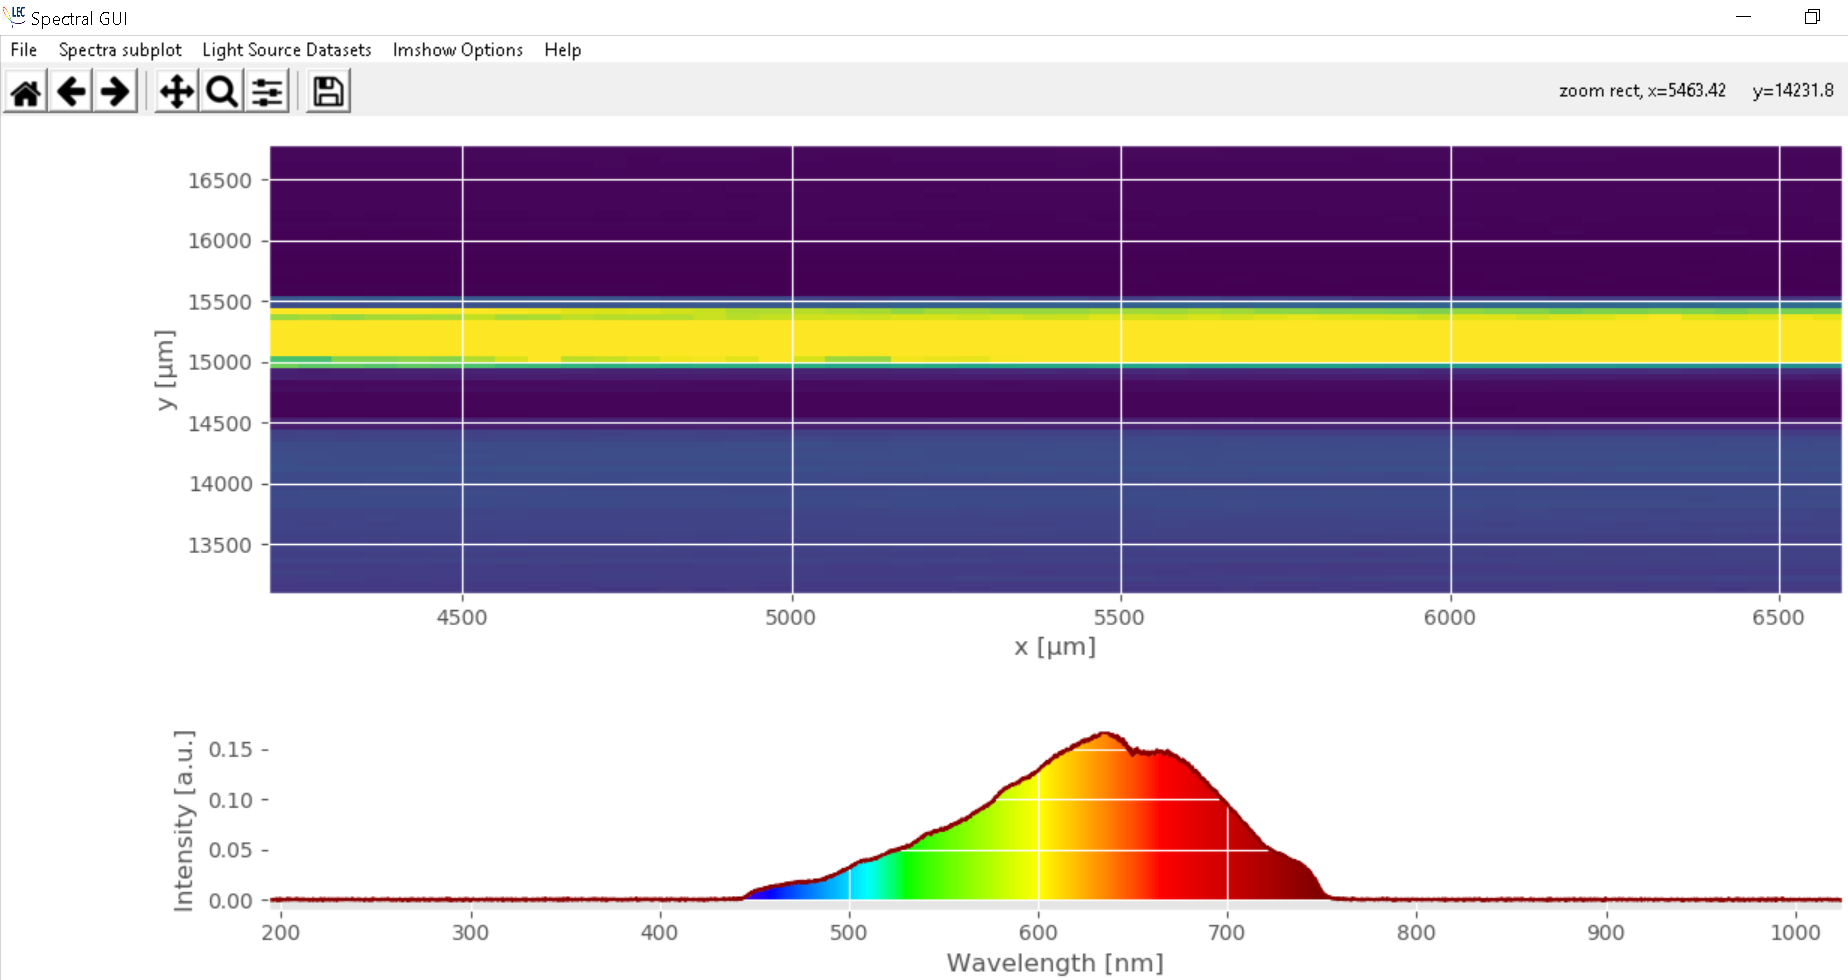
\includegraphics[width=1.0\textwidth]{Figs/microespectrometro/chidisp.png}
	\caption{Interfaz gráfica con el \textit{imshow} del $\chi^{2}$ de cada banda. \textit{Zoom} sobre el cromo que separa la banda pancromática de la banda verde.}
	\label{fig:GUI01}
\end{figure}

La interfaz gráfica permite además graficar el espectro de un cierto píxel de la imagen generada a partir de la selección con el mouse, guardar imágenes de la región de interés, mostrar el espectro de la fuente de luz utilizada, etc, todas opciones que se consideraron útiles para la caracterización de las propiedades ópticas del filtro y deseadas para el prototipo final del equipo.

El prototipo preliminar permitió establecer las características deseadas del equipo final y evaluar su factibilidad sin incurrir en gastos importantes de prototipado. Ahora bien, debido a la falta de resolución óptica no se obtuvo ningún resultado concluyente ya que este prototipo resultó una prueba de concepto. A este prototipo se le propusieron las siguientes mejoras que fueron incluidas en el montaje y construcción del microespectrómetro [\ref{sec:montcontmsp}]:

\begin{enumerate}
\justifying
\item \texttt{Fuente de luz [\ref{sec:fteluzyesp}]}: Se modificó la fuente de luz de \textit{Fiber-Lite} que consiste de un \textit{fiber bundle} (arreglo de fibras ópticas) de un diámetro de 4.8 mm por una fuente de luz acoplada con una fibra óptica multimodo cuya apertura numérica fue de 0.22 y cuyo diámetro del \textit{core} fue de 200 $\mu m$. Como no se contó con un objetivo adicional para enfocar la fuente de luz sobre el filtro y mediante un arreglo óptico elegir el tamaño del \textit{spot} incidente sobre el filtro , se decidió optar por la fuente de luz cuya salida divergente tuviera el menor ángulo del cono de luz de salida. Este criterio de diseño tenía como objetivo disminuir la región iluminada del filtro por la fuente de luz, lo que reduciría ciertas reflexiones espurias en los componentes ópticos del microespectrómetro provenientes de la luz de regiones no alcanzadas por el área de adquisición del microespectrómetro. Este efecto que aumenta proporcionalmente a la relación entre el área iluminada y el área adquirida del filtro se denomina efecto de Schwarzchild-Villiger \cite{Naora279} debería ser considerado en las futuras mejoras del equipo aquí propuesto ya que distorsiona el espectro de la región original que se quiere medir. Además la nueva fuente de luz utilizada tenía la misma fibra óptica que el espectrómetro, hecho que permitió realizar fácilmente la identificación de la región medida con el espectrómetro respecto de la imagen adquirida con la cámara web (Ver Sección \ref{sec:camwebgui}).
\item \texttt{Platina [\ref{sec:platina}]}: Como la plataforma motorizada de Thorlabs utilizada en el prototipo preliminar tenía un límite de recorrido de 13 mm x 13 mm, no se podía adquirir el espectro de transmisión del filtro completo cuya región que contiene a las cinco bandas tiene unas dimensiones de 27 mm x 25 mm. En consecuencia se desarrolló una platina motorizada con el suficiente recorrido para poder realizar el barrido completo del filtro y también se consideró el paso y precisión mecánicas mínimas como para poder adquirir áreas de defectos de diámetro mayor a 20$\mu m$ con la mayor cantidad de puntos posible.
\item \texttt{Microespectrómetro [\ref{sec:disop}-\ref{sec:softadq}]}: Se montó e incorporó al prototipo un microespectrómetro con una resolución óptica lateral diseñado para caracterizar defectos de diámetro mayor a 20 $\mu m$.
\item \texttt{Integración de una cámara web [\ref{sec:camwebgui}]}: Se incorporó una cámara \textit{web} y un  \textit{joystick} al equipo para poder seleccionar la región del filtro a medir y se desarrolló una interfaz gráfica para poder visualizar en simultáneo la imagen digital de dicha región y el espectro de transmisión. 
\end{enumerate}

%%%%%%%%%%%%%%%%%%%%%%%%%%%%%%%%%%%%%%%%%%%%%%%%%%%%%%%%%%%%%%%%%%%%%%%%%%%%%%%%%%%%%%%%%%%%%%%%%%%%%%%%%%%%%%%%%%%%%%%%%%%%%%%%%%%%%%%%%%%%%%%%%%%%%%%%%%%%%%%%%%%%%%%%%%%%%%%%%%%%%%%%%%%%%%%%%%%%%%%%%%%%%%%%%%%%%%%%%%%%
\singlespacing
\section{Diseño y construcción del microespectrómetro}
\label{sec:montcontmsp}
\spacing{1.5}

\hspace{0.5cm}En esta sección se describen los criterios de diseño y todas las consideraciones técnicas del microespectrómetro, de la platina motorizada desarrollada que fue controlada con un \textit{joystick} y de la cámara \textit{web} integrada. El equipo final desarrollado puede ser fácilmente adaptable a requerimientos ópticos y mecánicos específicos distintos a los presentados en esta tesis.
%%%%%%%%%%%%%%%%%%%%%%%%%%%%%%%%%%%%%%%%%%%%%%%%%%%%%%%%%%%%%%%%%%%%%%%%%%%%%%%%%%%%%%%%%%%%%%%%%%%%%%%%%%%%%%%%%%%%%%%%%%%%%%%%%%%%%%%%%%%%%%%%%%%%%%%%%%%%%%%%%%%%%%%%%%%%%%%%%%%%%%%%%%%%%%%%%%%%%%%%%%%%%%%%%%%%%%%%%%%%

\singlespacing
\subsection{Fuente de luz y espectrómetro \href{https://github.com/jrr1984/defects_analysis/blob/master/light_sources_spectrum.py}{\faGithub}}
\label{sec:fteluzyesp}
\spacing{1.5}

\hspace{0.5cm}El criterio de elección de la fuente de luz dependió fundamentalmente del rango de longitudes de onda que se quiso medir, que para el caso del filtro aquí analizado dicho rango se encontró entre los 450 nm y los 900 nm.
Se utilizó una fuente de luz halógena y de tungsteno modelo \href{https://www.thorlabs.com/newgrouppage9.cfm?objectgroup_id=7269&pn=SLS201L/M}{SLS201L} del fabricante Thorlabs. El espectro de emisión de dicha fuente de luz medido con el espectrómetro modelo \href{https://www.thorlabs.com/thorproduct.cfm?partnumber=CCS200/M#ad-image-0}{CCS200/M} del fabricante Thorlabs se muestra en el gráfico de la intensidad en función de la longitud de onda de la Figura \ref{fig:espfth}.

\begin{figure}[H]
	\centering
	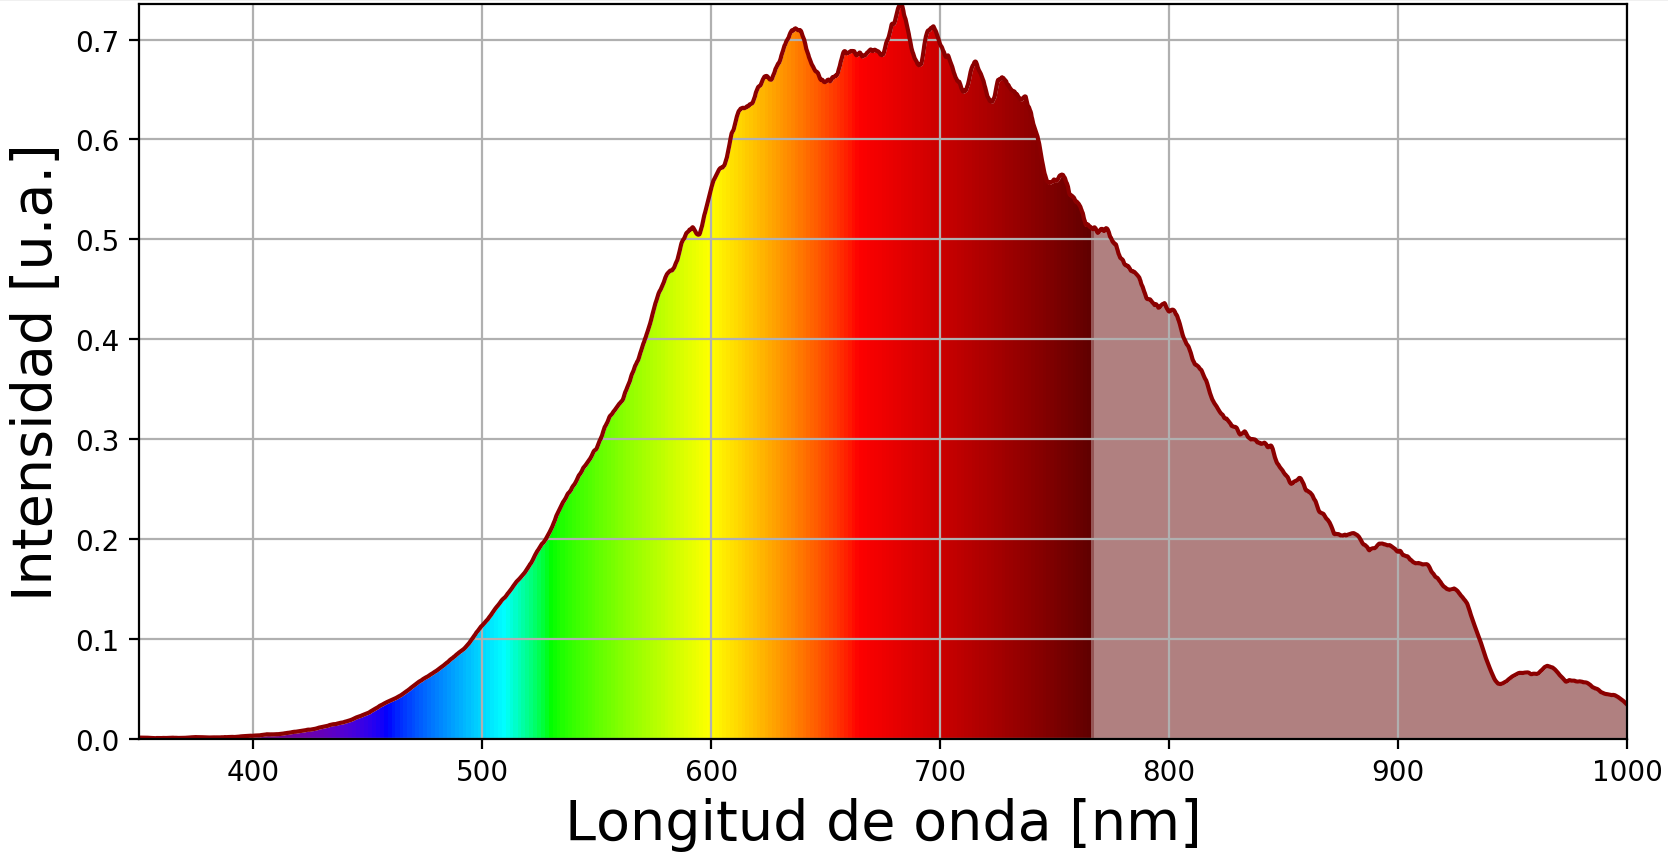
\includegraphics[width=1.0\textwidth]{Figs/microespectrometro/espfuentethorl.png}
	\caption{Espectro de emisión de la fuente de luz \href{https://www.thorlabs.com/newgrouppage9.cfm?objectgroup_id=7269&pn=SLS201L/M}{SLS201L} del fabricante Thorlabs [\href{https://github.com/jrr1984/defects_analysis/blob/master/light_sources_spectrum.py}{\faGithub}].}
	\label{fig:espfth}
\end{figure}

El espectro de emisión de la fuente de luz reportado por el fabricante indica que debería ser en el rango de longitudes de onda de 360 - 2600 nm, lo cual se pudo verificar por lo menos en el rango comprendido entre los 200 nm y los 1000 nm que es el rango de detección del espectrómetro. El fabricante reportó una precisión del espectrómetro menor a los 2 nm y el tiempo de integración del detector puede ser entre los 10 $\mu s$ y los 60 s.

Además de considerar el espectro de emisión de la fuente de luz otro parámetro importante resultó la potencia de radiación de la misma ya que en función de ésta se eligen los tiempos de integración del espectrómetro para tener una buena relación señal-ruido. En consecuencia, una lámpara de mayor potencia reduce los tiempos de medición, lo que haría al método de inspección con el microespectrómetro más compatible con los tiempos de duración de los procesos industriales. La potencia de radiación de la lámpara reportada por el fabricante fue de 10mW. 
%%%%%%%%%%%%%%%%%%%%%%%%%%%%%%%%%%%%%%%%%%%%%%%%%%%%%%%%%%%%%%%%%%%%%%%%%%%%%%%%%%%%%%%%%%%%%%%%%%%%%%%%%%%%%%%%%%%%%%%%%%%%%%%%%%%%%%%%%%%%%%%%%%%%%%%%%%%%%%%%%%%%%%%%%%%%%%%%%%%%%%%%%%%%%%%%%%%%%%%%%%%%%%%%%%%%%%%%%%%%

\singlespacing
\subsection{Platina \href{https://github.com/jrr1984/open\_frame\_XYStage}{\faGithub} \href{https://github.com/jrr1984/open_frame_XYStage/tree/master/3dprintedparts}{\faCubes}}
\label{sec:platina}
\spacing{1.5}

\hspace{0.5cm}Se desarrolló una platina de microscopía con dos grados de libertad para poder desplazar el filtro lateral y verticalmente respecto de la fuente de luz y del microespectrómetro para poder medir el espectro de transmisión del filtro en distintas regiones del mismo. Una imagen representativa de una de las primeras versiones de la platina con dos grados de libertad se muestra en la Figura \ref{fig:plato0}.


\begin{figure}[H]
	\centering
	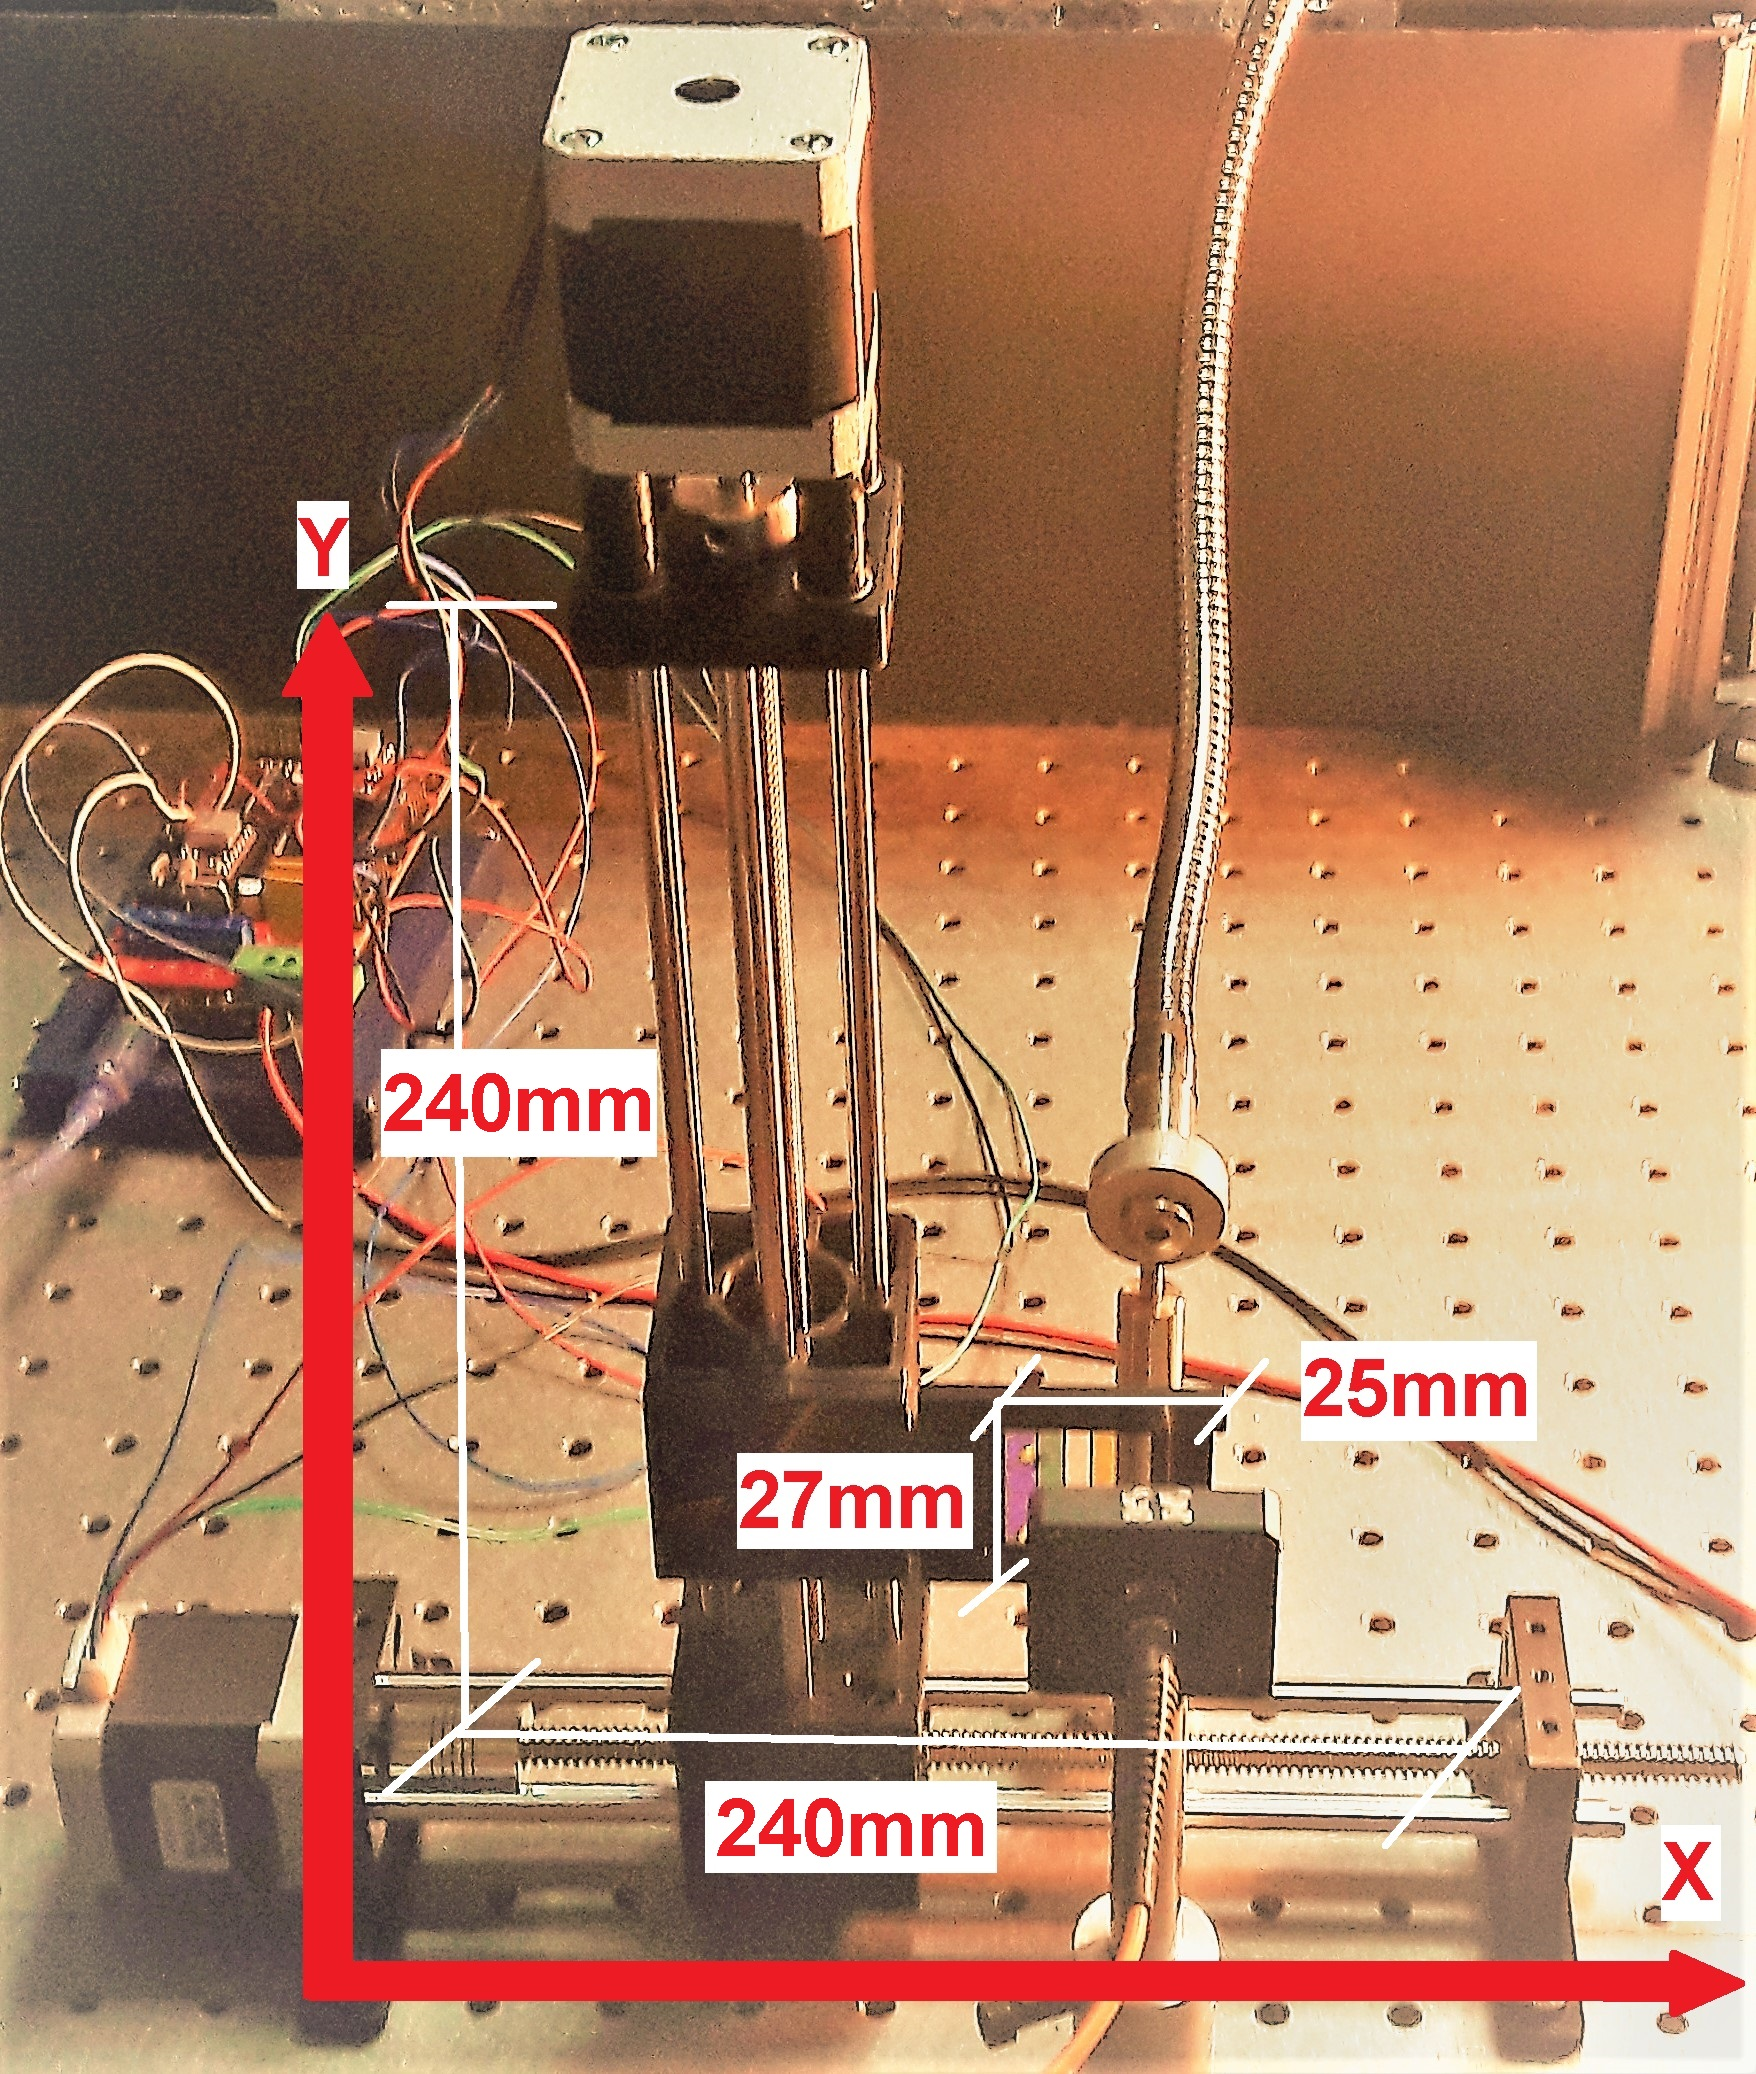
\includegraphics[scale=0.15]{Figs/microespectrometro/stageearly.jpg}
	\caption{Imagen de una de las primeras versiones de la platina motorizada con dos grados de libertad.}
	\label{fig:plato0}
\end{figure}


La construcción y desarrollo de la platina motorizada del microespectrómetro consistió de las siguientes etapas de prototipado:

\begin{enumerate}
\item Investigación previa de la literatura sobre platinas de microscopía de bajo costo y factibles para integrar al prototipo.
\item Elección de los componentes y materiales en función de la oferta local en Argentina.
\item De acuerdo a lo anterior se realizó un dimensionamiento de la platina y se determinó el recorrido total de cada uno de los grados de libertad. Esto permitió evaluar la factibilidad y aplicabilidad de la plataforma a desarrollar.
\item En conjunto con el diseñador industrial Federico Armesto se diseñaron las piezas de impresión 3D y se montó el primer eje de la platina. Se desarrolló la electrónica y el \textit{software} necesarios.
\item Una vez optimizado el diseño del primer eje, se montó el segundo eje de la platina. Se extendió el software y se integraron finales de carrera.
\item El prototipo de la platina seguía siendo actualizada al momento de escribir esta tesis.
\end{enumerate}

A continuación se describen algunas consideraciones técnicas y de diseño que se tuvieron en cuenta para el desarrollo de la platina motorizada y que podrían ser de utilidad para otros laboratorios que quisieran replicar la plataforma que aquí se presenta, realizar una adaptación ó simplemente como fuente de consulta.

%%%%%%%%%%%%%%%%%%%%%%%%%%%%%%%%%%%%%%%%%%%%%%%%%%%%%%%%%%%%%%%%%%%%%%%%%%%%%%%%%%%%%%%%%%%%%%%%%%%%%%%%%%%%%%

\begin{enumerate}
\item \texttt{Investigación previa de la literatura sobre platinas de microscopía de bajo costo y factibles para integrar al prototipo:}
\end{enumerate}

Respecto de la revisión de la literatura sobre platinas de microscopía de bajo costo y factibles para el prototipo, se consultaron  los prototipos cuyos proyectos hayan sido desarrollados bajo la modalidad \textit{open source} tanto para la distribución del diseño de las piezas 3D como del \textit{software}, dentro de las cuales se destacan \cite{schaa}(\textit{LabView}, EUR 250) y \cite{campbells}(Instrucciones vía puerto serie en \textit{Matlab} y \textit{python}, USD 1000). Dichas propuestas son también denominadas en cierto contexto DIY (\textit{Do it yourself}) ya que contienen toda la documentación y herramientas necesarias para que cualquier usuario con presupuesto y acceso a los mismos componentes pueda reproducir el proyecto. Además de estos proyectos se consultaron múltiples platinas de microscopía comerciales, donde en sus páginas \textit{web} la mayoría de los fabricantes distribuyen los planos de diseño, las piezas 3D libres para modificar, etc (\href{https://www.thorlabs.com/newgrouppage9.cfm?objectgroup\_id=2132}{NRT150 Thorlabs} USD 2456 x 2, \href{https://www.edmundoptics.com/p/150mm-motorized-stage/16419/}{\#59-747 EO} USD 2095 x 2). Ahora bien, hasta la fecha de escritura de este trabajo no se registraban prototipos de platinas motorizadas de microscopía desarrolladas en laboratorios del país como la que aquí se presenta por lo cual por medio de la presente se comparten las piezas de diseño 3D y el \textit{software} necesarios para poder replicarla y extender sus prestaciones. El costo total aproximado de la platina aquí desarrollada fue de USD 200.

\begin{enumerate}
  \setcounter{enumi}{1}
  \item \texttt{Elección de los componentes y materiales en función de la oferta local en Argentina.}
\end{enumerate}

El tipo de platina motorizada a desarrollar depende del presupuesto, de la oferta local de los componentes y de los requerimientos mecánicos de precisión, longitud de recorrido y repetibilidad que se tengan. Estos tres conceptos se encontraban relacionados fuertemente entre sí. Si bien se podrian haber comprado los componentes de la platina en el exterior del país, la futura necesidad de comprar nuevamente alguno de los componentes debido al desgaste ó rotura de los mismos, hacen de esta implementación de la compra una mala práctica del prototipado. En este sentido se eligieron componentes masivos en el país, los cuales se puedan conseguir fácilmente sus repuestos en caso de necesidad. Al mismo tiempo, los componentes masivos son los que tienen un menor costo debido a su mayor demanda.

A modo de referencia pero no de publicidad se consultaron fundamentalmente tres proveedores de componentes mecánicos y de electrónica, de la ciudad de Buenos Aires y de la provincia de Buenos Aires: \href{https://3dinsumos.com.ar/}{3DInsumos} (Caseros,pcia. de Buenos Aires), \href{https://ingia.com.ar/}{Ingia Automatización}(Saavedra, C.A.B.A.) y \href{https://candy-ho.com/}{Candy-Ho} (Villa Martelli, C.A.B.A.). A partir de la oferta de estos y otros proveedores se eligieron los componentes de la platina tomando como idea de diseño e implementación la platina de \cite{schaa} que por su bajo costo, la utilización de piezas 3D lo que facilitan el prototipado rápido (dependiendo de la disponibilidad de una impresora 3D), hacían de esa propuesta la más indicada para ser implementada.

Los componentes principales de la platina son el motor paso a paso y el sistema de transmisión que transforma la rotación del motor en un desplazamiento lineal. Uno de los sino el motor paso a paso más popular del mercado es el \href{https://www.pololu.com/product/1200}{NEMA 17} que es ampliamente utilizado en impresoras 3D y CNC de medianos requerimientos de torque. Por este motivo se eligió ese motor en lugar del \href{https://www.pololu.com/product/1204}{NEMA 8} utilizado en \cite{schaa}, que sólo se podía conseguir haciendo un pedido al exterior lo que encarece su costo y alarga notablemente los tiempos de prototipado.

De la familia de motores paso a paso NEMA 17 (Ver Figura \ref{fig:nema17}) existen distintos modelos dependiendo los requerimientos de torque y de resolución fundamentalmente. El torque no fue una limitante para la elección del modelo con lo cual en función del mismo se priorizó el de menor precio. Ahora bien, respecto de la precisión existen dos modelos con pasos mínimos de rotación de 1.8 grados y de 0.9 grados, con lo cual se tienen 200 y 400 pasos por revolución respectivamente. Se evaluó la oferta disponible en el mercado y se eligió un NEMA 17 con un paso mínimo de 0.9 grados con el fin de obtener la mayor resolución en el desplazamiento lineal, a pesar de que costo era mayor.

A la elección del motor, le sigue la elección del sistema de transmisión donde existen múltiples opciones dependiendo de la precisión, entre ellas las correa dentadas con poleas, las varillas roscadas, los husillos de bolas, etc. De acuerdo a \cite{schaa} se optó por una varilla roscada masiva en el mercado del tipo \href{https://www.mcmaster.com/acme-screws/acme-lead-screws-and-nuts/}{ACME} (Ver Figura \ref{fig:acmea}) con un paso (\textit{pitch}) de 2 mm, es decir que por cada revolución completa del motor se completa un desplazamiento lineal de 2 mm y un diámetro de 8 mm. La rotación del motor paso a paso es transferida a la varilla roscada ACME por medio de un acople sólido con agujeros para prisioneros M3 equidistanciados a 180° para que la varilla roscada quede centrada, que fue diseñado (Ver \href{https://github.com/jrr1984/open_frame_XYStage/blob/master/3dprintedparts/acopleRIGIDO.STL}{\faCubes}). Además del sistema de transmisión se tuvo que elegir un sistema de desplazamiento que es el que permite el movimiento de los ejes de la platina. Se eligió la opción más utilizada en impresoras 3D en el que se utilizan sistemas lineales con barras rectificadas de acero de 6mm de diámetro y rodamientos lineales \href{https://uk.misumi-ec.com/vona2/detail/221000091678/?HissuCode=LM6LUU}{LM6LUU}.

\begin{figure}[H]
	\begin{floatrow}
		\ffigbox{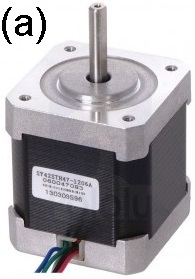
\includegraphics[scale=0.7]{Figs/microespectrometro/nema17.jpg}}{\caption{Motor paso a paso \href{https://www.pololu.com/product/1200}{NEMA 17} con una resolución de 400 pasos por revolución (0.9° por paso).}\label{fig:nema17}}
		\ffigbox{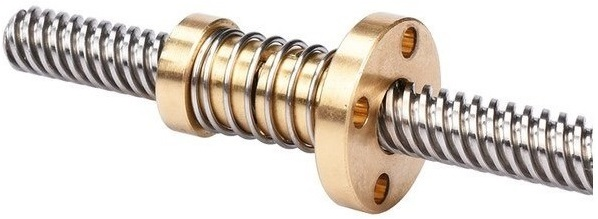
\includegraphics[scale=0.7]{Figs/microespectrometro/acmeantib.jpg}}{ \caption{Varilla roscada del tipo \href{https://www.mcmaster.com/acme-screws/acme-lead-screws-and-nuts/}{ACME} con un paso (\textit{pitch}) de 2 mm  y un diámetro de 8 mm, junto con una tuerca \textit{anti-backslash}}\label{fig:acmea}}
	\end{floatrow}
\end{figure}

La resolución espacial es la mínima distancia de recorido en cualquiera de los ejes de desplazamiento de la platina. La misma viene dada por la siguiente ecuación:
\begin{equation}
\text{Resolución} [\mu m] = \frac{\text{\textit{Pitch} del ACME}}{\text{\# de pasos por revolución del motor}} = \frac{2 mm}{400 pasos} = \frac{5 \mu m}{paso}
\end{equation}

Además esta resolución puede ser modificada por medio de la electrónica que controla los motores paso a paso aplicando una técnica que se conoce como \textit{microstepping} \cite{7806244}. Esta técnica permite al motor realizar rotaciones de ángulos menores al paso mínimo del motor, con lo cual se mejora la resolución ya que se puede subdividir un paso completo del motor en 2,4,8,16 e incluso hasta en 32 pasos (teóricos). Al mismo tiempo se reduce el ruido del motor y el movimiento del mismo se suaviza. La técnica es impelementada por el controlador de corriente que utiliza un algoritmo que a su salida envía una modulación sinusoidal y discreta de la corriente, donde cada paso de esa función sinusoidal consiste de un micropaso y el período de la señal es igual al paso completo original del motor.

Los dos controladores de corriente de los motores paso a paso más populares con la capacidad de aplicar \textit{microstepping} son el \href{https://www.pololu.com/product/2133}{DRV8825}(hasta 32 micropasos y 2.5 A) y el \href{https://www.pololu.com/product/1182}{A4988} (hasta 16 micropasos y 2 A). Se eligió finalmente para la platina el \textit{driver} A4988 (Ver Figura \ref{fig:a4988}) y se limitó la máxima corriente que podía entregar de acuerdo al consumo observado de los motores en condiciones de operación normales, ajustando el potenciómetro (Ver Figura \ref{fig:a4988}) a partir de la medición de una tensión de referencia de acuerdo a las especificaciones del manual del fabricante \cite{a4988}.

Se eligió un \href{https://store.arduino.cc/usa/mega-2560-r3}{\textit{Arduino MEGA 2560}} para controlar la lógica de la platina vía el puerto USB de una computadora y se le montó a los pines hembra del arduino un \textit{shield} \href{https://reprap.org/wiki/RAMPS_1.4}{\textit{RAMPS 1.4}} donde se colocaron los \textit{drivers} de los motores, las conexiones de los finales de carrera y el \textit{joystick}. La RAMPS fue alimentada de forma independiente con una fuente de tensión.

\begin{figure}[H]
    \begin{floatrow}
        \ffigbox{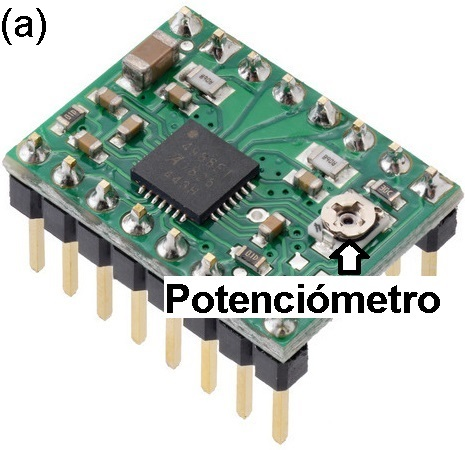
\includegraphics[scale=0.5]{Figs/microespectrometro/a4988.jpg}}{\caption{Controlador de los motores paso a paso A4988.}\label{fig:a4988}}
        \ffigbox{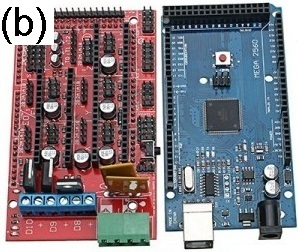
\includegraphics[scale=1.4]{Figs/microespectrometro/megaramps.jpg}}{ \caption{\href{https://store.arduino.cc/usa/mega-2560-r3}{\textit{Arduino MEGA 2560}} a la derecha en azul y \href{https://reprap.org/wiki/RAMPS_1.4}{\textit{Shield RAMPS 1.4}} a la izquierda en rojo. }\label{fig:ramps}}
    \end{floatrow}
\end{figure}

%%%%%%%%%%%%%%%%%%%%%%%%%%%%%%%%%%%%%%%%%%%%%%%%%%%%%%%%%%%%%%%%%%%%%%%%%%%%%%%%%%%%%%%%%%%%%%%%%%%%%%%%%%%%%%

\begin{enumerate}
  \setcounter{enumi}{2}
  \item \texttt{De acuerdo a lo anterior se realizó un dimensionamiento de la platina y se determinó el recorrido total de cada uno de los grados de libertad. Esto permitió evaluar la factibilidad y aplicabilidad de la plataforma a desarrollar.}
\end{enumerate}

Antes de realizar la compra de los componentes necesarios para montar el primer eje se determinó el recorrido total de cada uno de los grados de libertad de la platina de acuerdo a la oferta de los proveedores. Por ejemplo, existen comercialmente distintas longitudes de varillas roscadas ACME y se eligió una longitud de la misma de 500 mm, de forma tal que al cortar dicha varilla se pueda obtener las dos varillas necesarias para cada eje de la platina, cada una de 250 mm de largo. El mismo razonamiento fue aplicado a las varillas de acero de 6mm de diámetro, para las cuales se compraron dos varillas de 1 metro que cada una fue cortada en cuatro partes de 250 mm cada una. De esta manera, se realizó un diagrama tentativo con el software \textit{Solidworks} de uno de los ejes de la platina como se muestra en la Figura \ref{fig:dimejee}, que fue siendo actualizando dependiendo las dimensiones de los componentes encontrados comercialmente.

\begin{figure}[H]
	\centering
	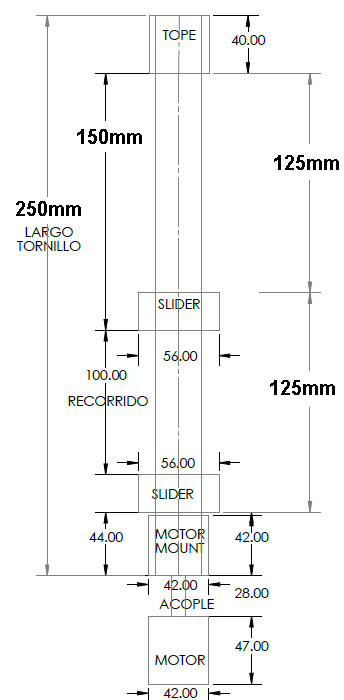
\includegraphics[scale=1.0]{Figs/microespectrometro/dimensio.png}
	\caption{Estimación del recorrido de uno de los ejes de la platina.}
	\label{fig:dimejee}
\end{figure}

El objetivo de esta etapa del prototipado es evaluar la factibilidad y aplicabilidad de la platina para poder desplazar al filtro respecto de la fuente de luz y del espectrómetro de manera tal de poder obtener una medición del espectro en cualquier región del filtro deseada. 

%%%%%%%%%%%%%%%%%%%%%%%%%%%%%%%%%%%%%%%%%%%%%%%%%%%%%%%%%%%%%%%%%%%%%%%%%%%%%%%%%%%%%%%%%%%%%%%%%%%%%%%%%%%%%%
\begin{enumerate}
  \setcounter{enumi}{2}
  \item \texttt{En conjunto con el diseñador industrial Federico Armesto se diseñaron las piezas de impresión 3D y se montó el primer eje de la platina. Se desarrolló la electrónica y el \textit{software} necesarios.}
\end{enumerate}





%%%%%%%%%%%%%%%%%%%%%%%%%%%%%%%%%%%%%%%%%%%%%%%%%%%%%%%%%%%%%%%%%%%%%%%%%%%%%%%%%%%%%%%%%%%%%%%%%%%%%%%%%%%%%%%%%%%%%%%%%%%%%%%%%%%%%%%%%%%%%%%%%%%%%%%%%%%%%%%%%%%%%%%%%%%%%%%%%%%%%%%%%%%%%%%%%%%%%%%%%%%%%%%%%%%%%%%%%%%%

\singlespacing
\subsection{Diseño óptico del microespectrómetro}
\label{sec:disop}
\spacing{1.5}

%%%%%%%%%%%%%%%%%%%%%%%%%%%%%%%%%%%%%%%%%%%%%%%%%%%%%%%%%%%%%%%%%%%%%%%%%%%%%%%%%%%%%%%%%%%%%%%%%%%%%%%%%%%%%%%%%%%%%%%%%%%%%%%%%%%%%%%%%%%%%%%%%%%%%%%%%%%%%%%%%%%%%%%%%%%%%%%%%%%%%%%%%%%%%%%%%%%%%%%%%%%%%%%%%%%%%%%%%%%%

\singlespacing
\subsection{Montaje y alineación preliminar del microespectrómetro}
\label{sec:montalin}
\spacing{1.5}

%%%%%%%%%%%%%%%%%%%%%%%%%%%%%%%%%%%%%%%%%%%%%%%%%%%%%%%%%%%%%%%%%%%%%%%%%%%%%%%%%%%%%%%%%%%%%%%%%%%%%%%%%%%%%%%%%%%%%%%%%%%%%%%%%%%%%%%%%%%%%%%%%%%%%%%%%%%%%%%%%%%%%%%%%%%%%%%%%%%%%%%%%%%%%%%%%%%%%%%%%%%%%%%%%%%%%%%%%%%%

\singlespacing
\subsection{Foco y resolución espacial del microespectrómetro}
\label{sec:focoresol}
\spacing{1.5}

\hspace{0.5cm}Para poner en foco el microespectrómetro sobre la cara externa del filtro más cerca al objetivo, se buscó el mínimo de la resolución espacial.

La resolución espacial se obtiene a partir del ajuste de las mediciones de una transición banda-cromo.

Para no alargar el tiempo de duración de las mediciones se mapeó el espectrómetro con la cámara. De lo contrario el único feedback que se tiene para saber si se está en una banda o en el cromo es la medición del espectro.

En consecuencia se conectó la fibra óptica montada sobre el cage destinado a medir con el espectrómetro, a la fuente de luz y por reflexión se observó en la adquisición en vivo de la cámara en qué posición de la imagen se observaba el haz de luz reflejado. Se centró dicho haz al centro de la cámara y de esa forma se determinó que el centro de la cámara está asociado con la medición efectiva del microespectrómetro. Se hace notar que la cámara no se encuentra en foco todavía, solo fue puesta aproximadamente a la misma distancia focal que la lente de tubo.

El setup para realizar este mapeo es el siguiente:
\begin{figure}[H]
	\centering
	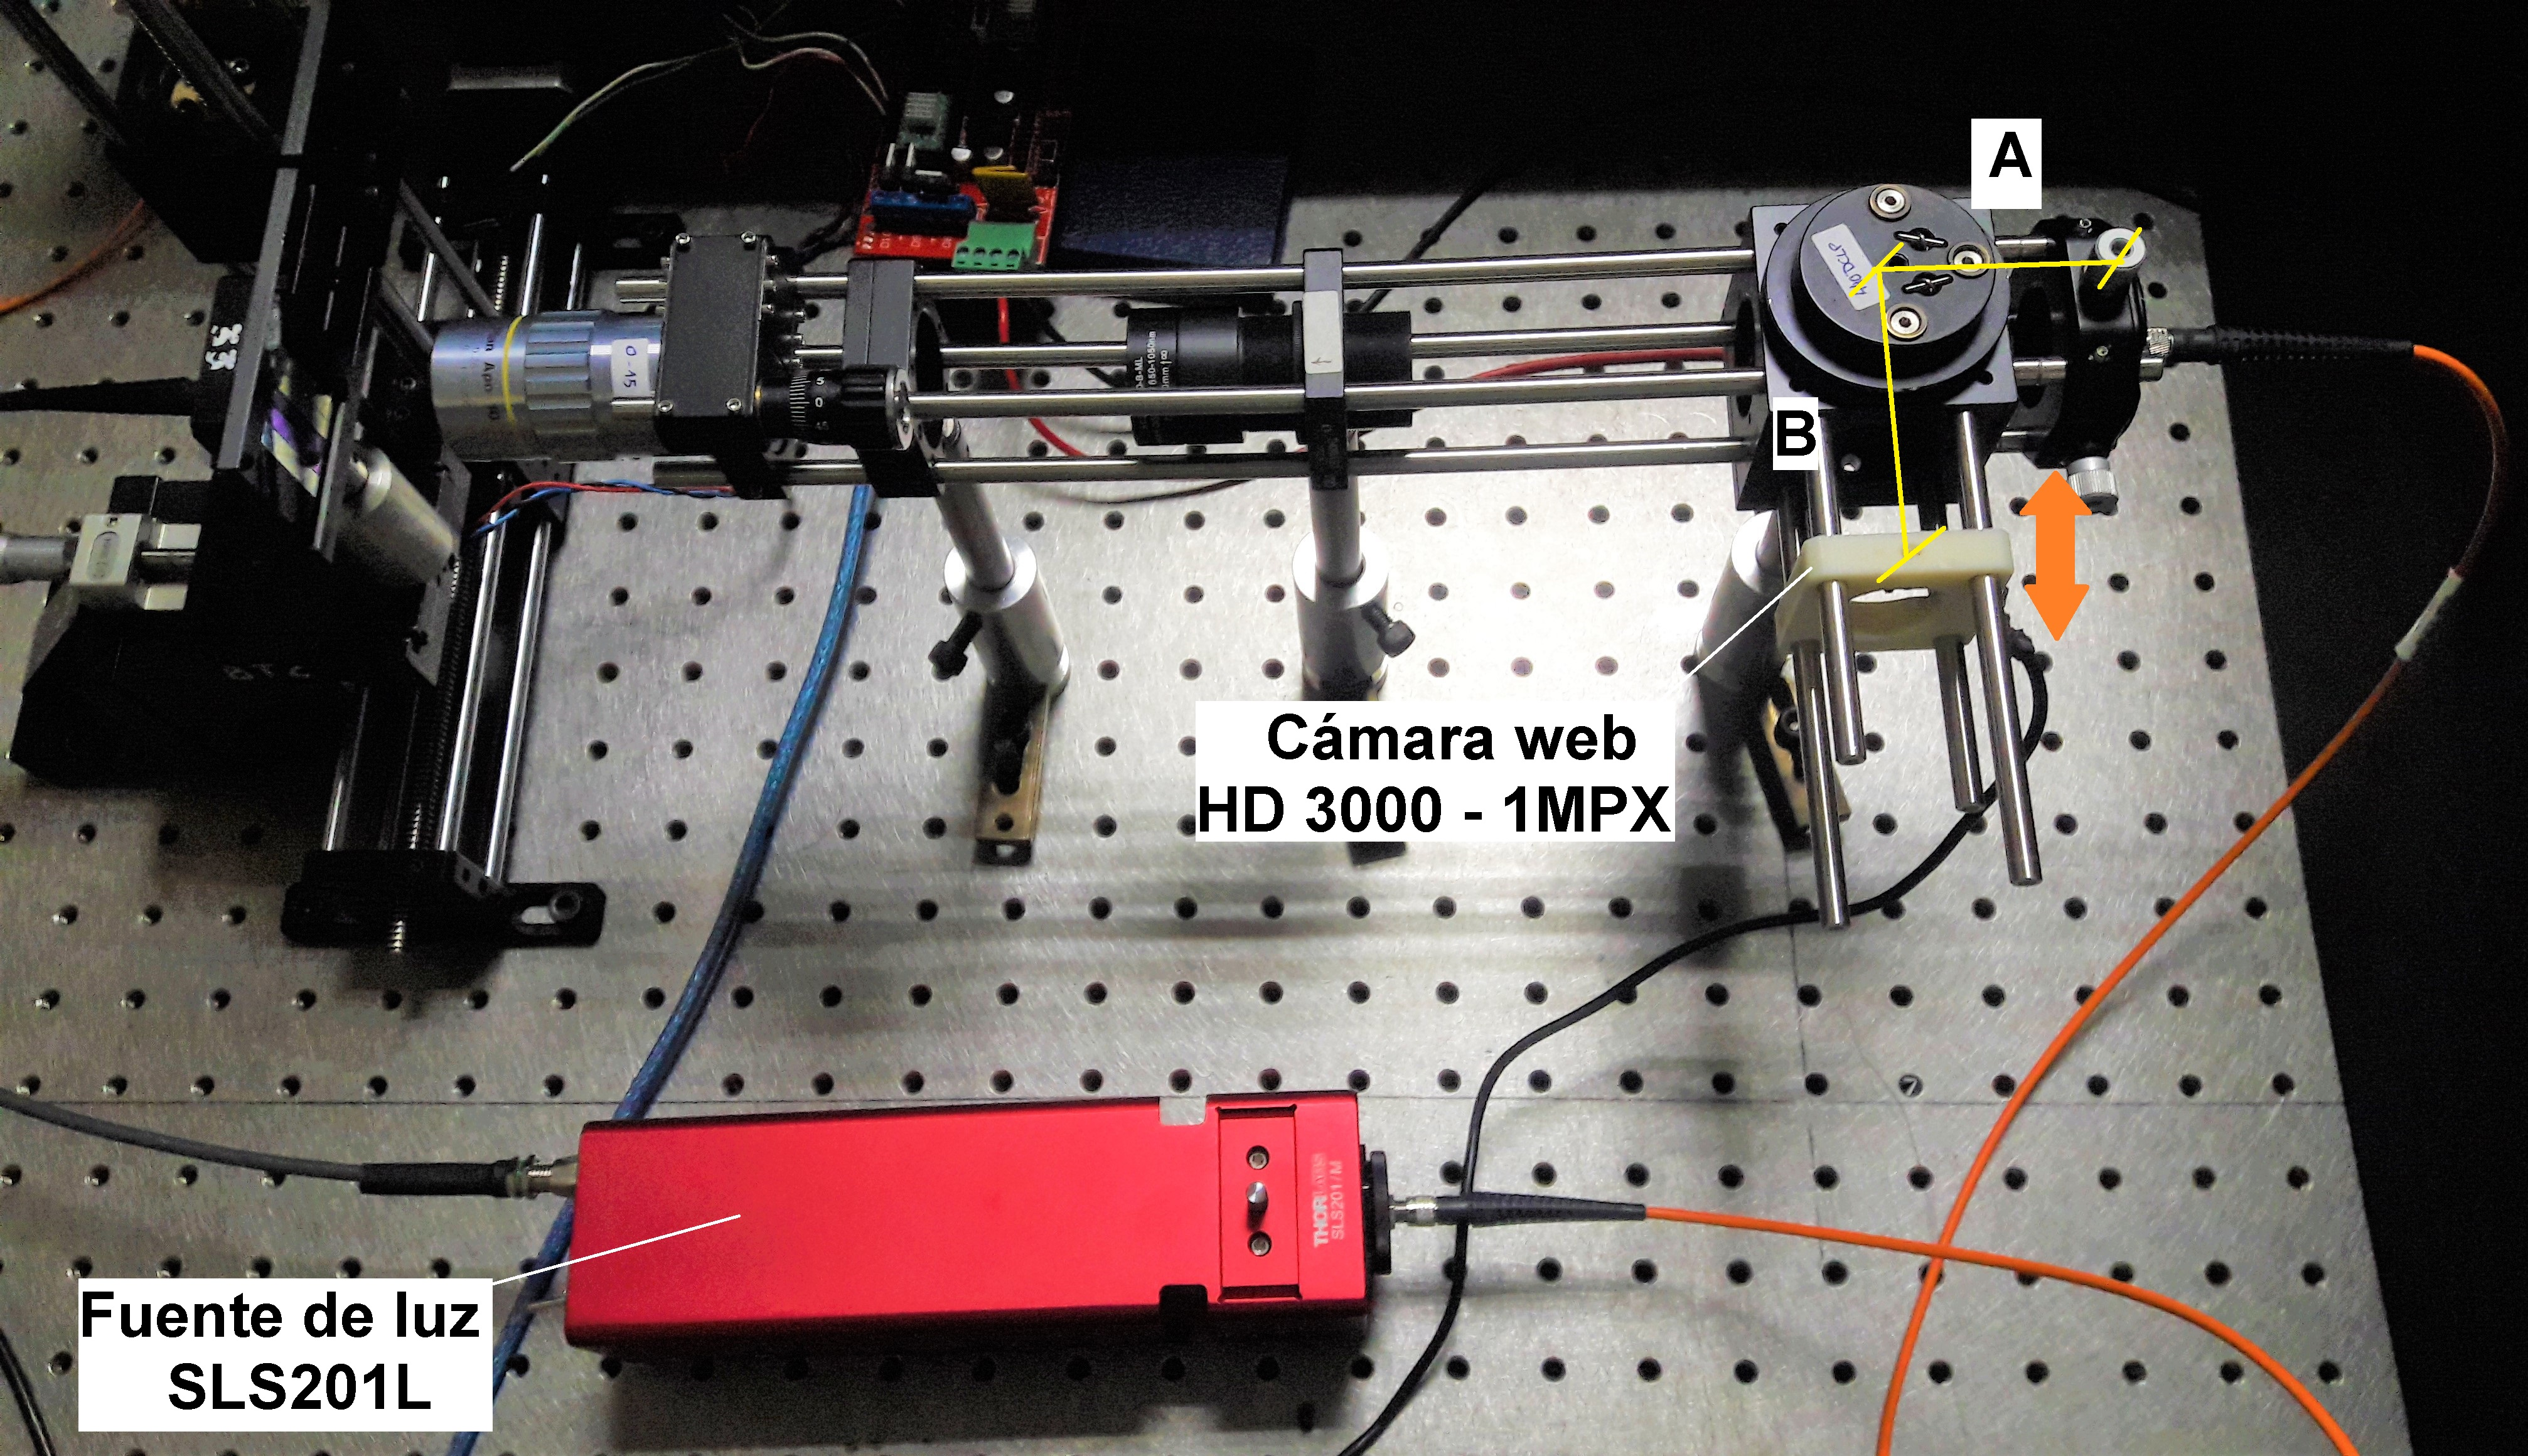
\includegraphics[scale=0.1]{Figs/microespectrometro/mapespeccam.jpg}
	\caption{Setup para mapear el espectrómetro con la cámara.}
	\label{fig:bgcel}
\end{figure}


Con los tornillos de la tapa de arriba del beamsplitter se puede ajustar en altura el beamsplitter para poder observar en el centro de la cámara la medición del espectrómetro.
\begin{figure}[H]
	\centering
	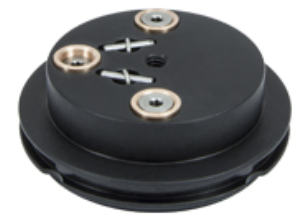
\includegraphics[scale=0.5]{Figs/microespectrometro/b4c.png}
	\caption{Tapa de arriba del beamsplitter.}
	\label{fig:bgcel}
\end{figure}


\begin{figure}[H]
	\centering
	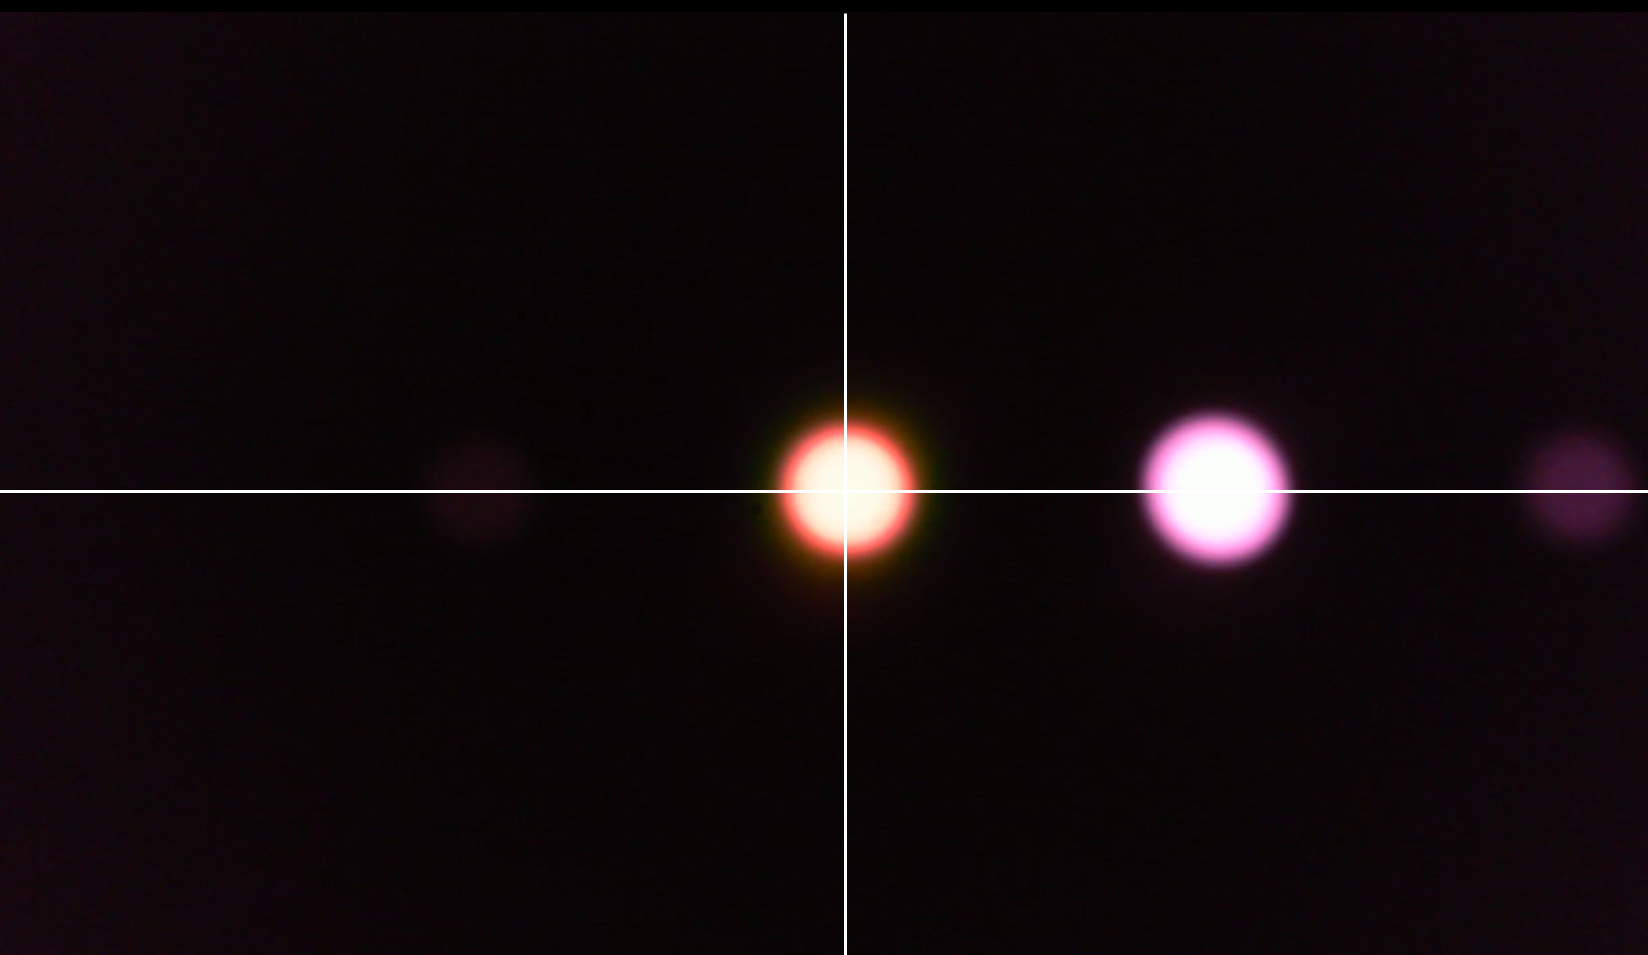
\includegraphics[scale=0.5]{Figs/microespectrometro/mapspectrometrocamera.png}
	\caption{Visualización en la cámara de la reflexión del filtro de la iluminación.}
	\label{fig:bgcel}
\end{figure}


No se tocó ni la cámara ni ninguna parte del setup a partir de ese momento para no perder este mapeo, a pesar de que la cámara no se encuentre perfectamente en foco (no hace falta probablemente poner una imagen de la cámara mostrando que no está en foco..), es decir que la imagen no se vea del todo nítida.
Luego se puso en foco el microespectrómetro.



\begin{figure}[H]
	\centering
	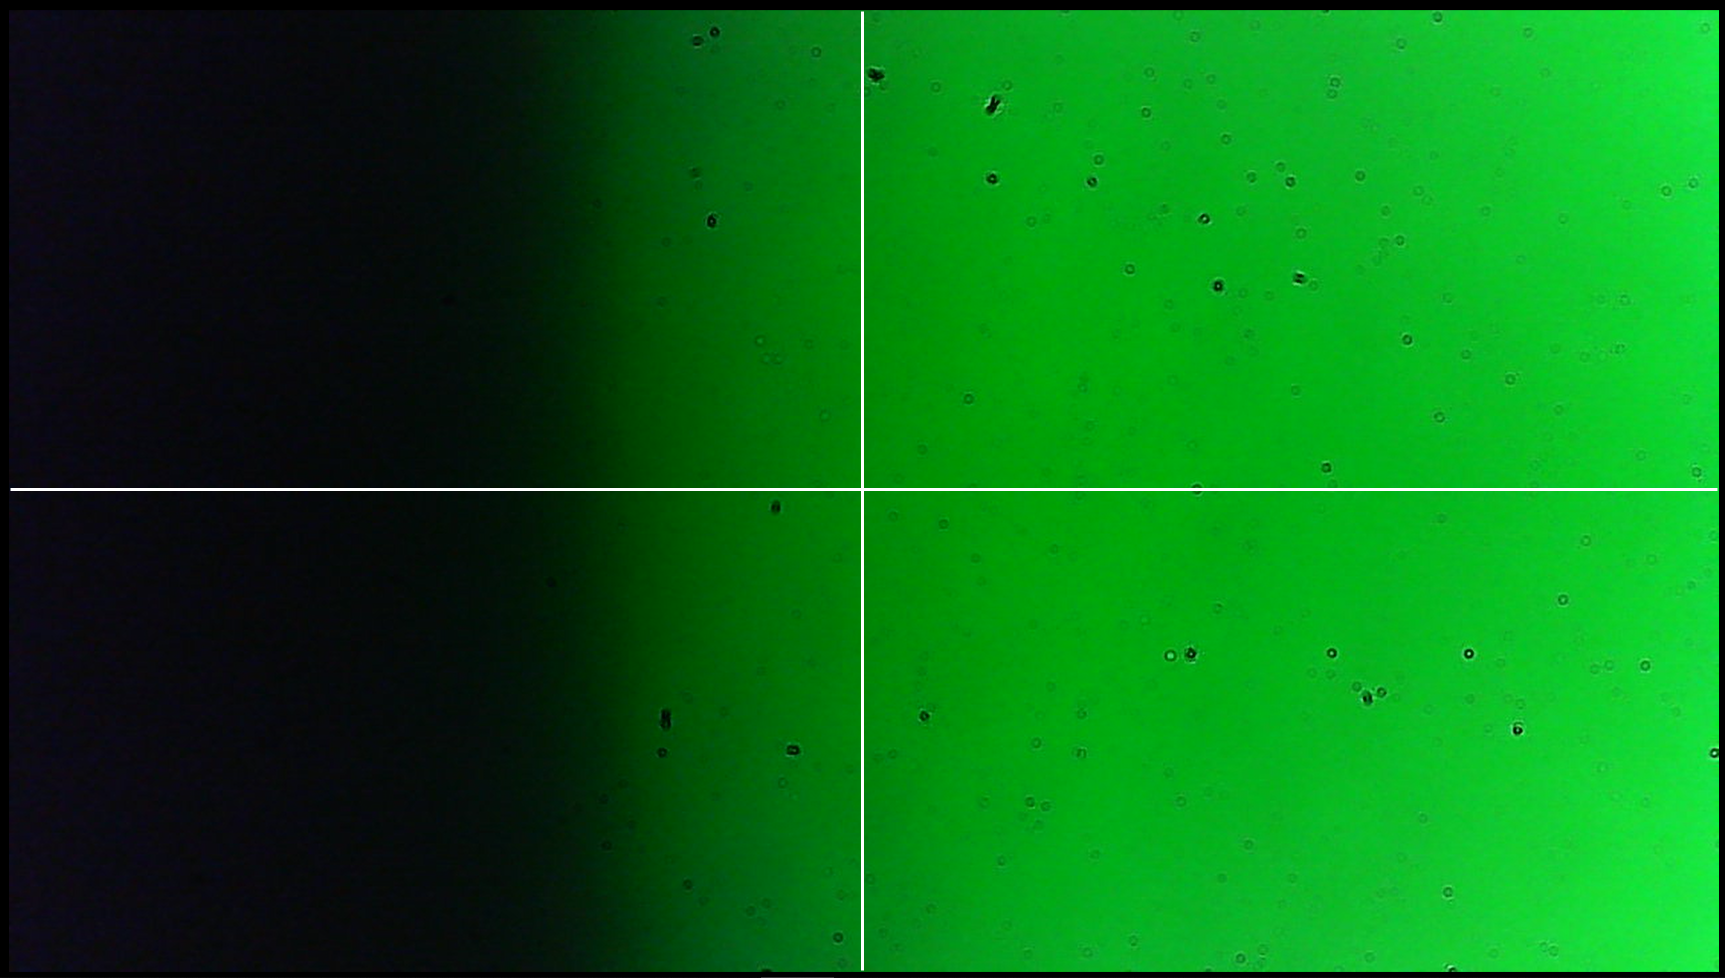
\includegraphics[scale=0.5]{Figs/microespectrometro/medtransicion.png}
	\caption{Visualización en la cámara de la reflexión del filtro de la iluminación.}
	\label{fig:bgcel}
\end{figure}


durante el experimento se tiene el feedback de cutelog:

\begin{figure}[H]
	\centering
	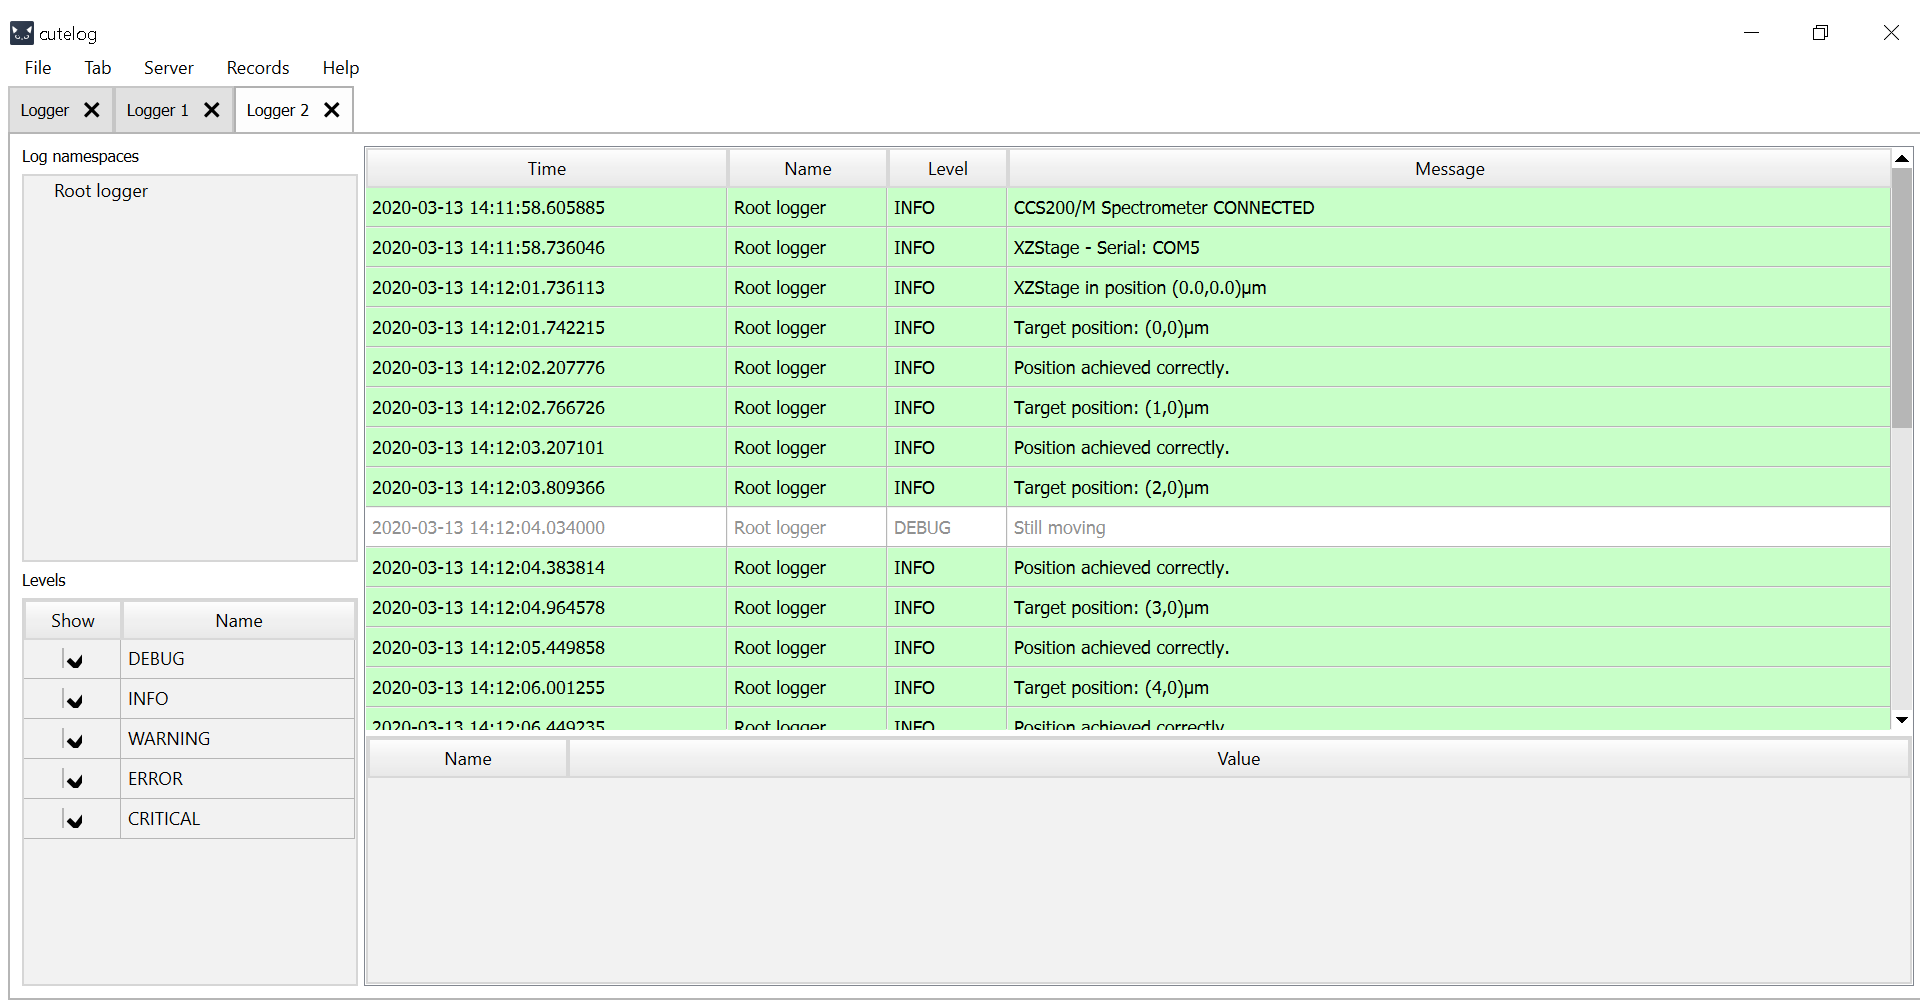
\includegraphics[scale=0.5]{Figs/microespectrometro/cutelog.png}
	\caption{Visualización en la cámara de la reflexión del filtro de la iluminación.}
	\label{fig:bgcel}
\end{figure}


\begin{figure}[H]
	\centering
	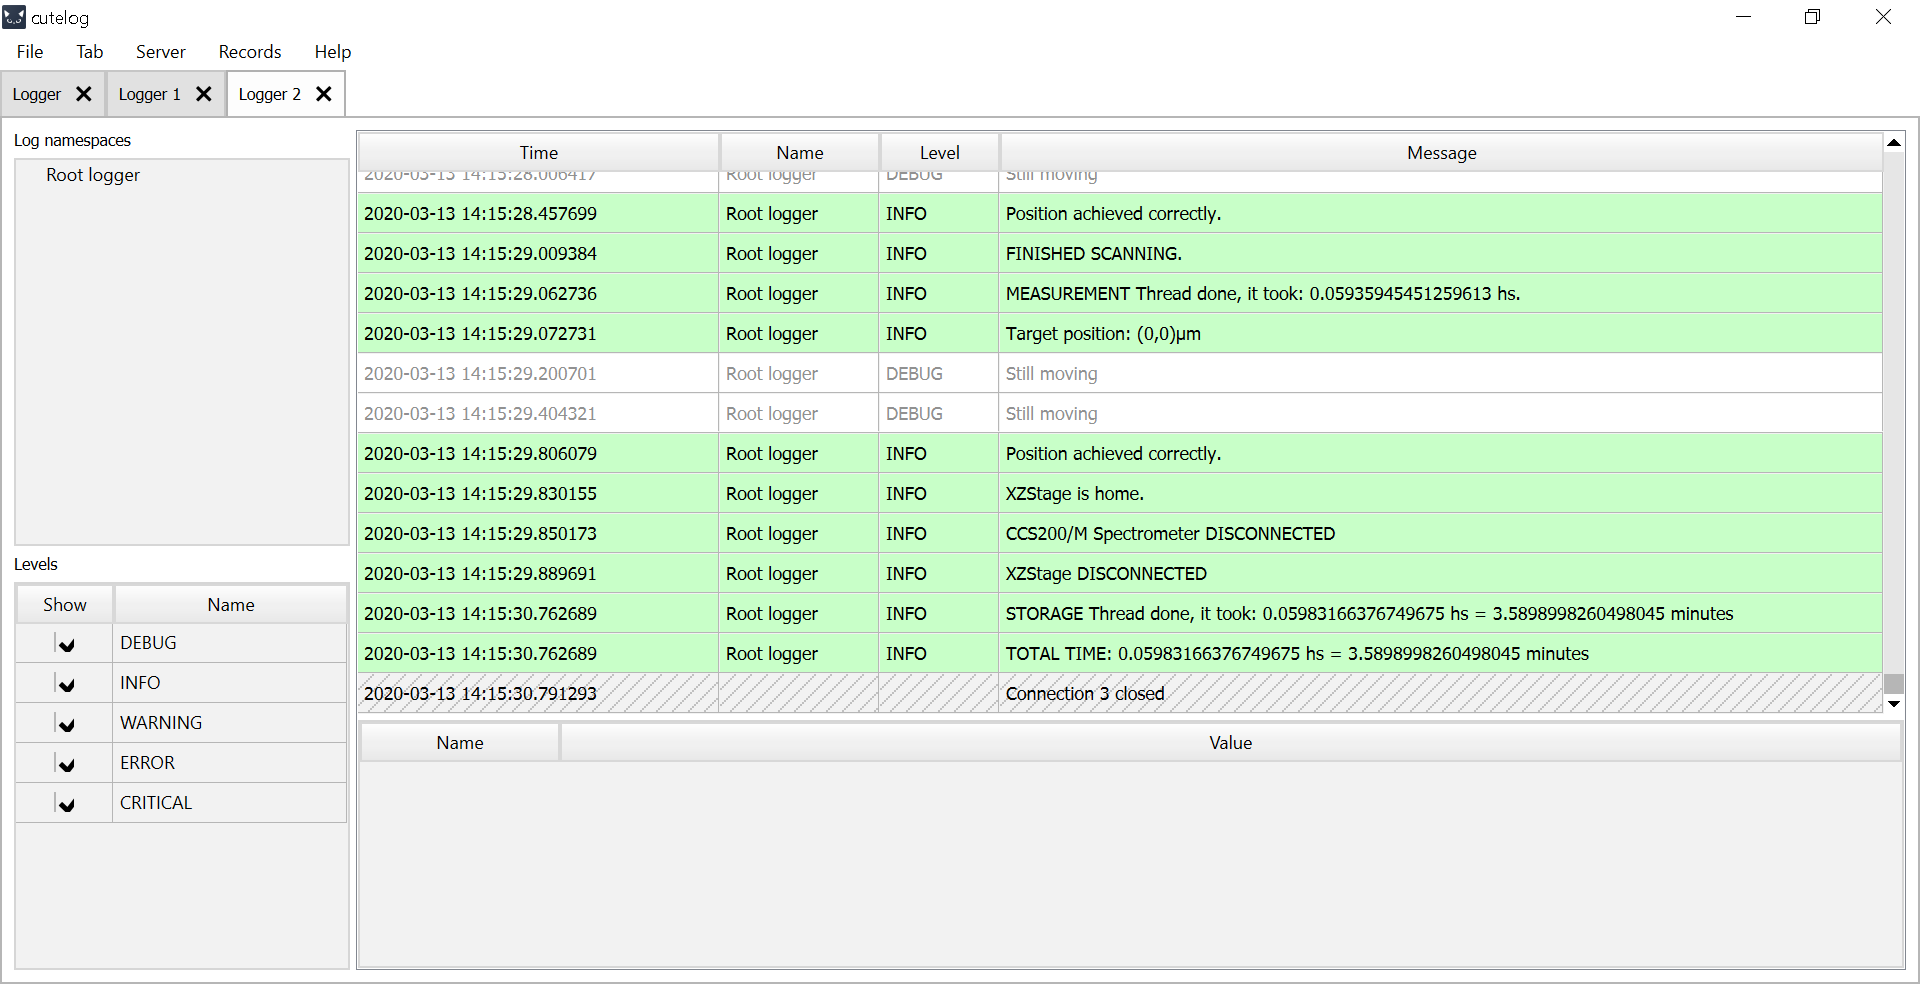
\includegraphics[scale=0.5]{Figs/microespectrometro/fincutelog.png}
	\caption{Visualización en la cámara de la reflexión del filtro de la iluminación.}
	\label{fig:bgcel}
\end{figure}


Las mediciones son ajustadas en matlab con una función error:
\begin{equation}
	(a/2)*erfc(sqrt(2)*(x-b)/c)
\end{equation}

\begin{figure}[H]
	\centering
	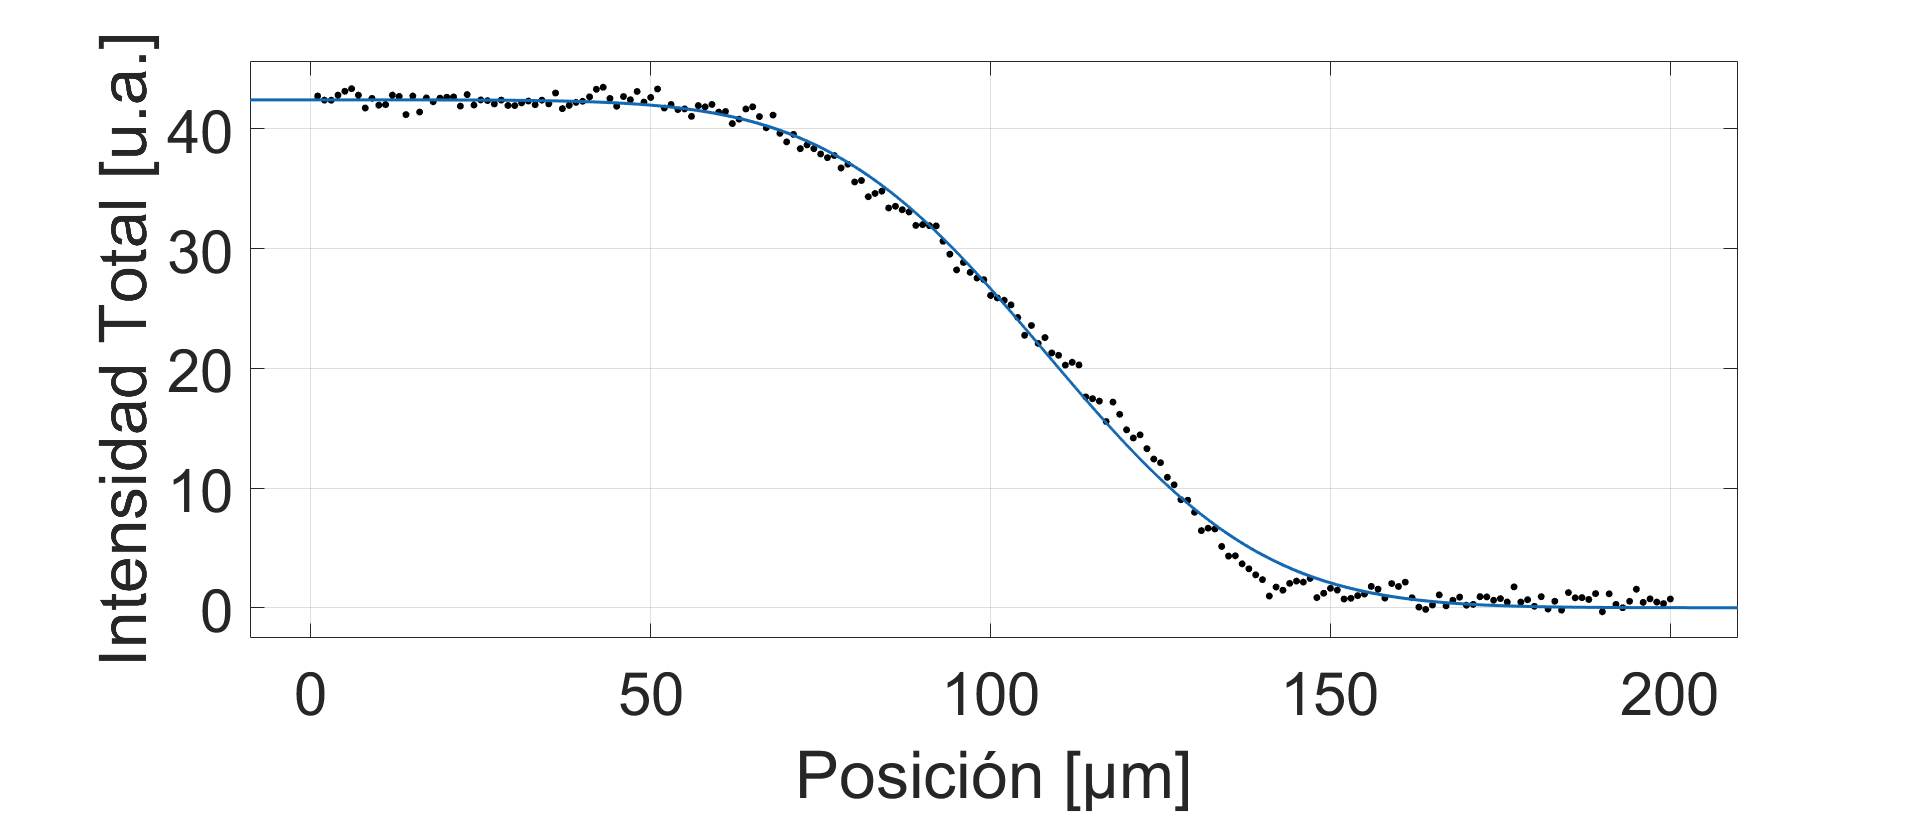
\includegraphics[scale=0.3]{Figs/microespectrometro/fit0.png}
	\caption{Visualización en la cámara de la reflexión del filtro de la iluminación.}
	\label{fig:bgcel}
\end{figure}

Resultados del ajuste:

General model:\par
$f(x) = (a/2)*erfc(sqrt(2)*(x-b)/c)$ \par
Coefficients (with 95$\%$ confidence bounds): \par
$a =       42.43  (42.2, 42.66)$\par
$b =       108.2  (107.8, 108.7)$\par
$c =       50.46  (49.25, 51.68)$\par

Goodness of fit:\par
SSE: 151.1\par
R-square: 0.9976\par
Adjusted R-square: 0.9976\par
RMSE: 0.8758\par

Luego moviendo la perilla del SM1Z para cambiar la distancia entre el objetivo y el filtro se repite la medición.


Comentar bien la siguiente foto, poner en la imagen que distancia se está variando, ettc
\begin{figure}[H]
	\centering
	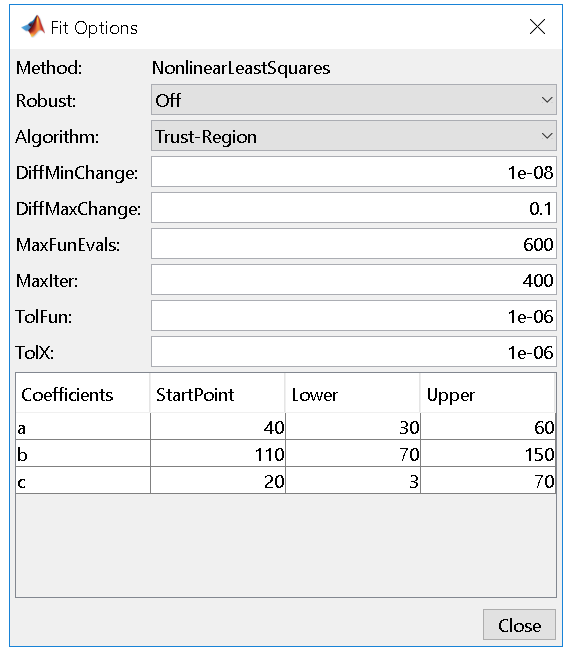
\includegraphics[scale=0.4]{Figs/microespectrometro/refinacionparam.png}
	\caption{Visualización en la cámara de la reflexión del filtro de la iluminación.}
	\label{fig:bgcel}
\end{figure}


Para hacer el ajuste se refinan los parámetros del modelo:

\begin{figure}[H]
	\centering
	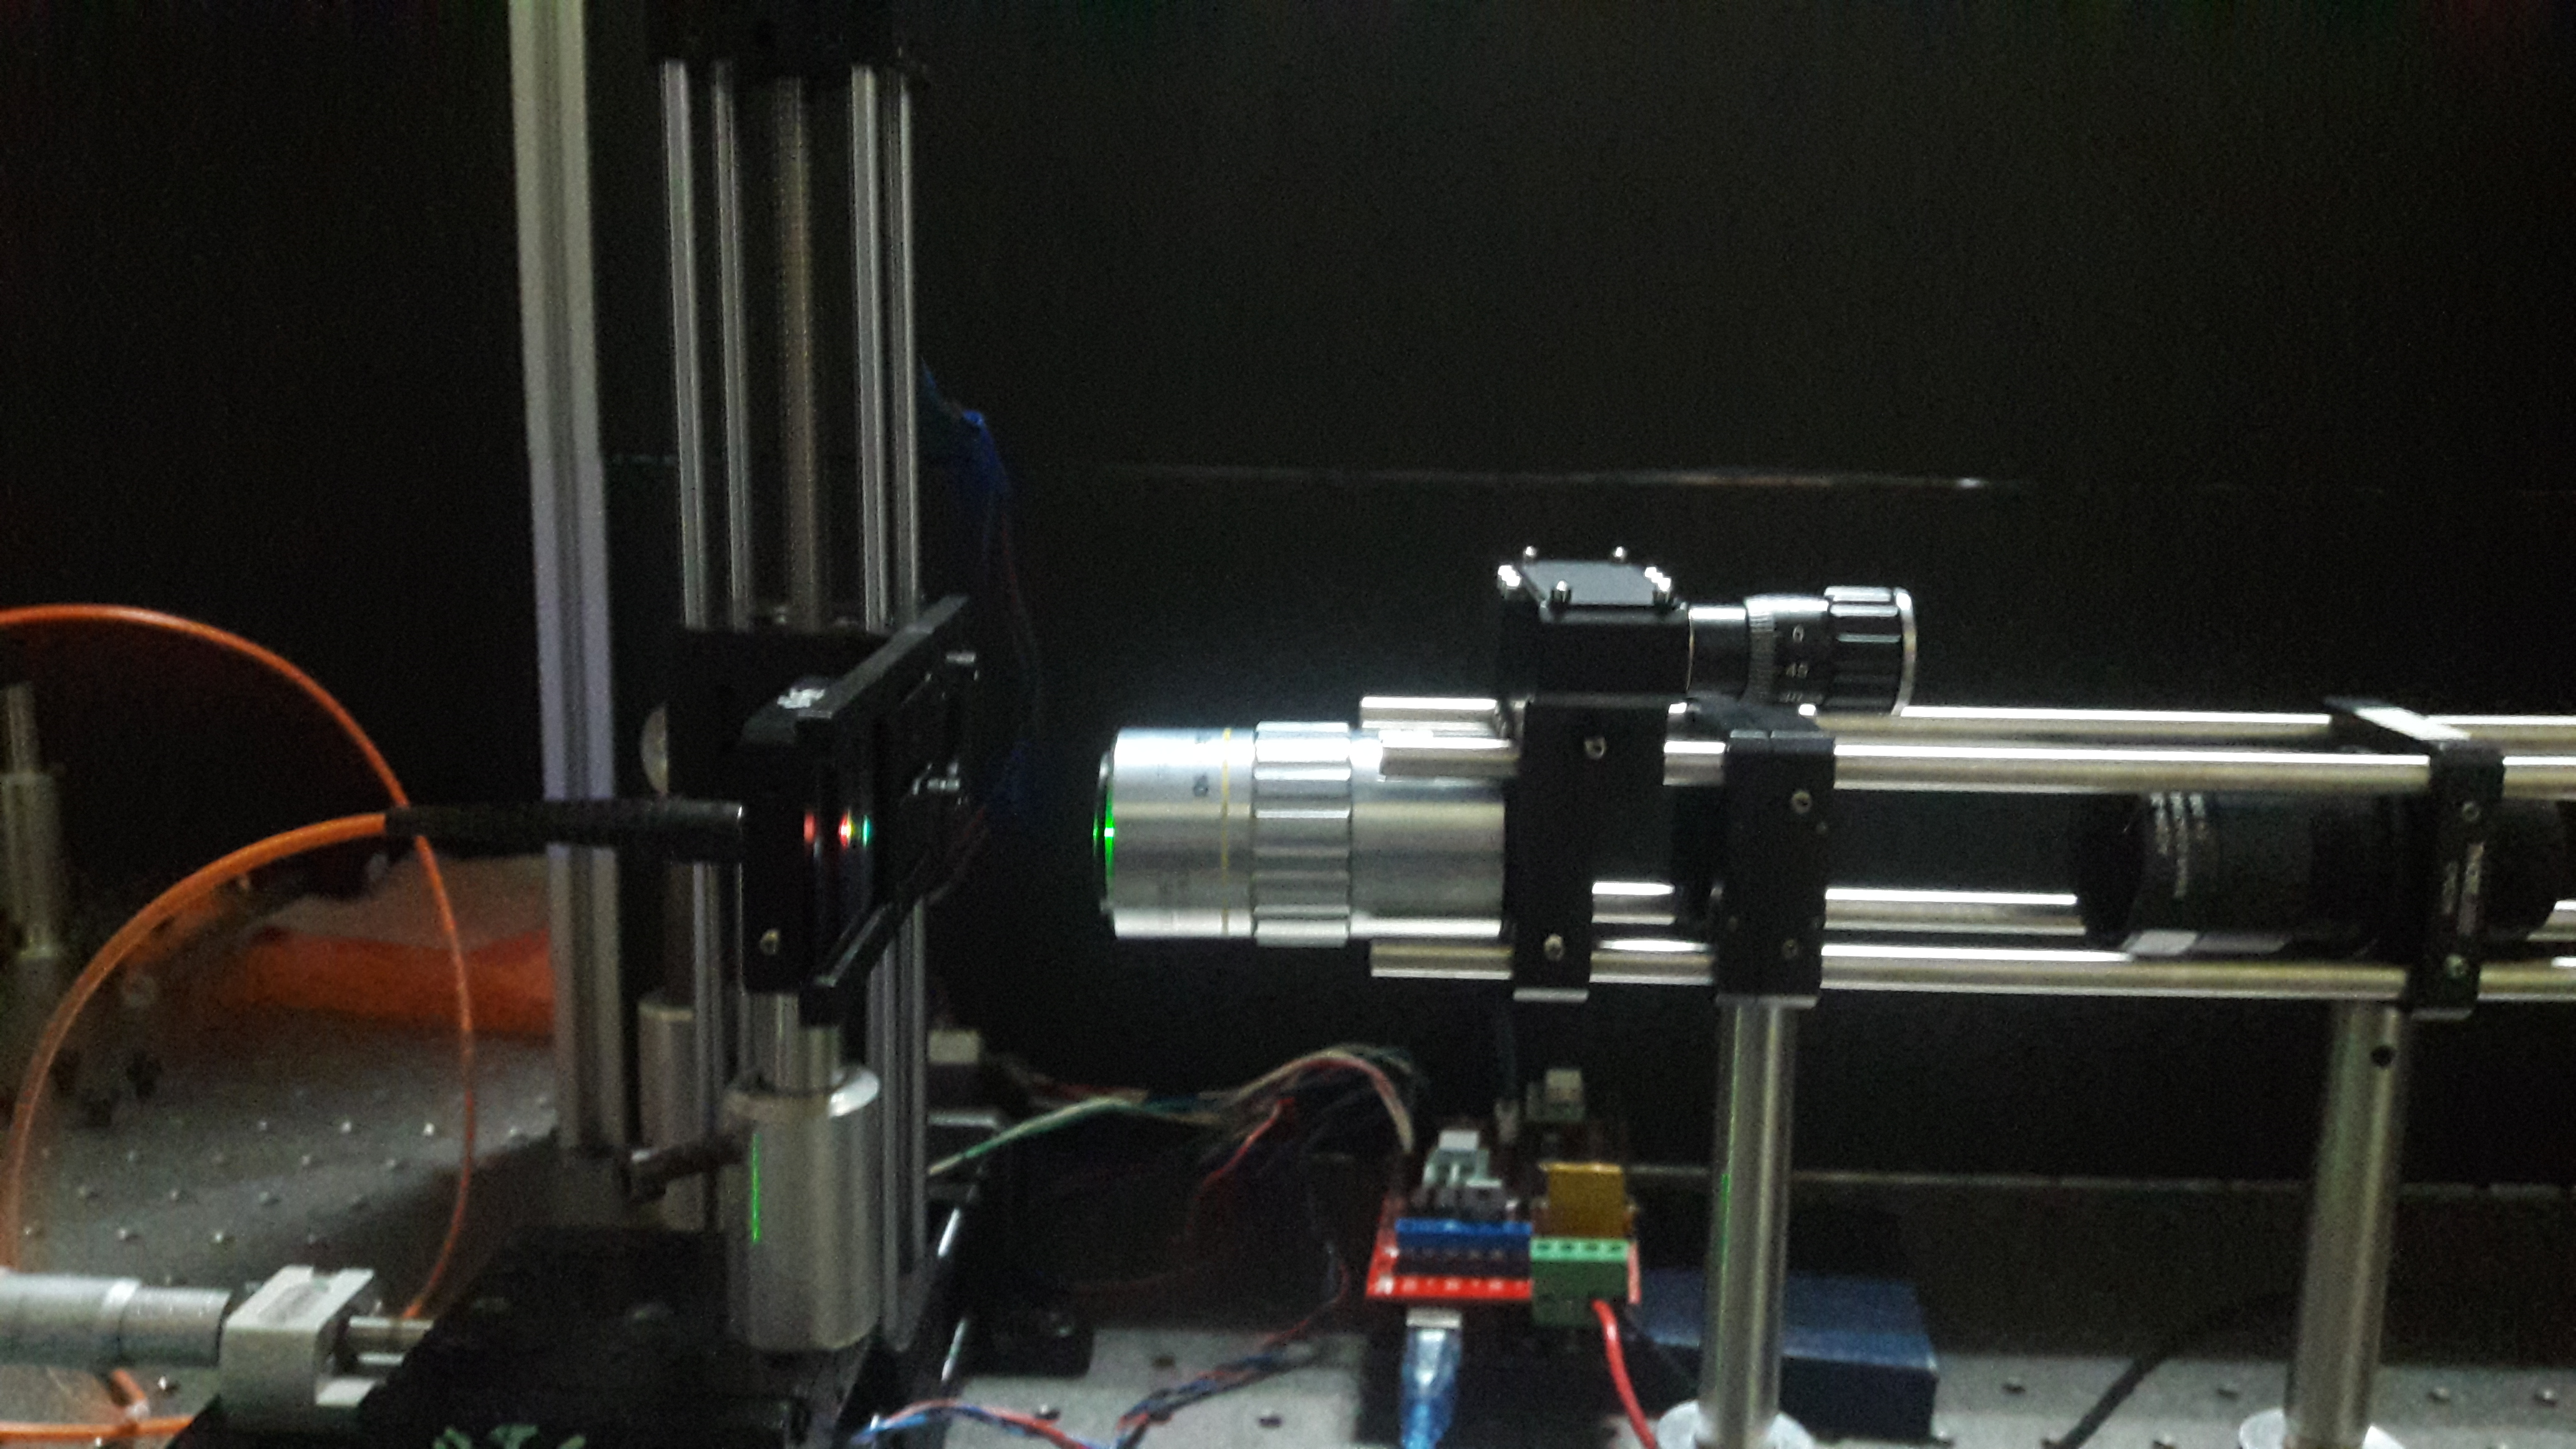
\includegraphics[scale=0.1]{Figs/microespectrometro/sm1zcambio.jpg}
	\caption{Visualización en la cámara de la reflexión del filtro de la iluminación.}
	\label{fig:bgcel}
\end{figure}


La idea es poner en foco el espectrómetro en alguna región del filtro, enfocar luego la cámara y después al mover el filtro a alguna otra región, tan solo hay que poner en foco el 'sistema' mirando la cámara. Al mismo tiempo si se quiere se puede volver a repetir el procedimiento de buscar el mínimo.


Gráfico de poner en foco el microespectrómetro: (19 de marzo)

mediciones guardadas en: data mediciones, simultaneidad, foco.

vamos recorriendo horario en pasos de 50 micrones en el SM1Z.
mediciones que consisten en un barrido de 80 micrones de largo, con pasos de 1 micron.. esto en la stage


RESULTADOS:

Z                  RESOLUCIÓN

0                  12.46 dudoso?

-50               13.5

-100             13.12

-150              12.87

-200              11.29

%%%%%%%%%%%%%%%%%%%%%%%%%%%%%%%%%%%%%%%%%%%%%%%%%%%%%%%%%%%%%%%%%%%%%%%%%%%%%%%%%%%%%%%%%%%%%%%%%%%%%%%%%%%%%%%%%%%%%%%%%%%%%%%%%%%%%%%%%%%%%%%%%%%%%%%%%%%%%%%%%%%%%%%%%%%%%%%%%%%%%%%%%%%%%%%%%%%%%%%%%%%%%%%%%%%%%%%%%%%%

\singlespacing
\subsection{\textit{Software} automatizado de adquisición}
\label{sec:softadq}
\spacing{1.5}

%%%%%%%%%%%%%%%%%%%%%%%%%%%%%%%%%%%%%%%%%%%%%%%%%%%%%%%%%%%%%%%%%%%%%%%%%%%%%%%%%%%%%%%%%%%%%%%%%%%%%%%%%%%%%%%%%%%%%%%%%%%%%%%%%%%%%%%%%%%%%%%%%%%%%%%%%%%%%%%%%%%%%%%%%%%%%%%%%%%%%%%%%%%%%%%%%%%%%%%%%%%%%%%%%%%%%%%%%%%%

\singlespacing
\subsection{Integración de una cámara web. Adquisición simultánea de imágenes y de espectros de transmisión mediante una interfaz gráfica \href{https://github.com/jrr1984/defectsGUI}{\faGithub}}
\label{sec:camwebgui}
\spacing{1.5}

%%%%%%%%%%%%%%%%%%%%%%%%%%%%%%%%%%%%%%%%%%%%%%%%%%%%%%%%%%%%%%%%%%%%%%%%%%%%%%%%%%%%%%%%%%%%%%%%%%%%%%%%%%%%%%%%%%%%%%%%%%%%%%%%%%%%%%%%%%%%%%%%%%%%%%%%%%%%%%%%%%%%%%%%%%%%%%%%%%%%%%%%%%%%%%%%%%%%%%%%%%%%%%%%%%%%%%%%%%%%

\singlespacing
\section{Aplicación del microespectrómetro a la caracterización de filtros multiespectrales}
\label{sec:resgrales}
\spacing{1.5}

%%%%%%%%%%%%%%%%%%%%%%%%%%%%%%%%%%%%%%%%%%%%%%%%%%%%%%%%%%%%%%%%%%%%%%%%%%%%%%%%%%%%%%%%%%%%%%%%%%%%%%%%%%%%%%%%%%%%%%%%%%%%%%%%%%%%%%%%%%%%%%%%%%%%%%%%%%%%%%%%%%%%%%%%%%%%%%%%%%%%%%%%%%%%%%%%%%%%%%%%%%%%%%%%%%%%%%%%%%%%

\singlespacing
\subsection{Espectro de transmisión de cada banda del filtro}
\label{sec:espectransm}
\spacing{1.5}

\hspace{0.5cm}Se midió el espectro de transmisión 


azul 
\begin{figure}[H]
	\centering
	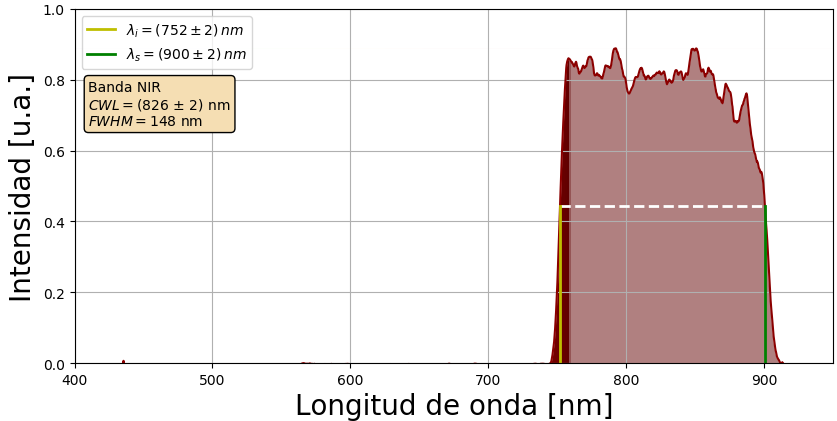
\includegraphics[width=1.0\textwidth]{Figs/microespectrometro/espectro_nir.png}
	\caption{Arreglo experimental del prototipo 0.}
	\label{fig:setup0}
\end{figure}

verde
\begin{figure}[H]
	\centering
	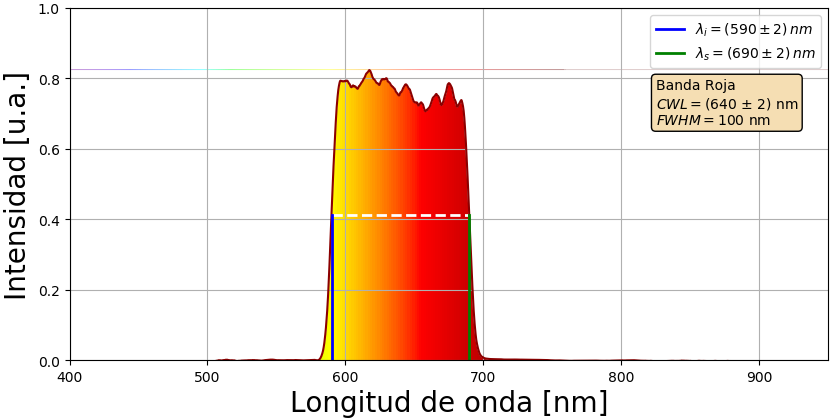
\includegraphics[width=1.0\textwidth]{Figs/microespectrometro/espectro_roja.png}
	\caption{Arreglo experimental del prototipo 0.}
	\label{fig:setup0}
\end{figure}

pancromática
\begin{figure}[H]
	\centering
	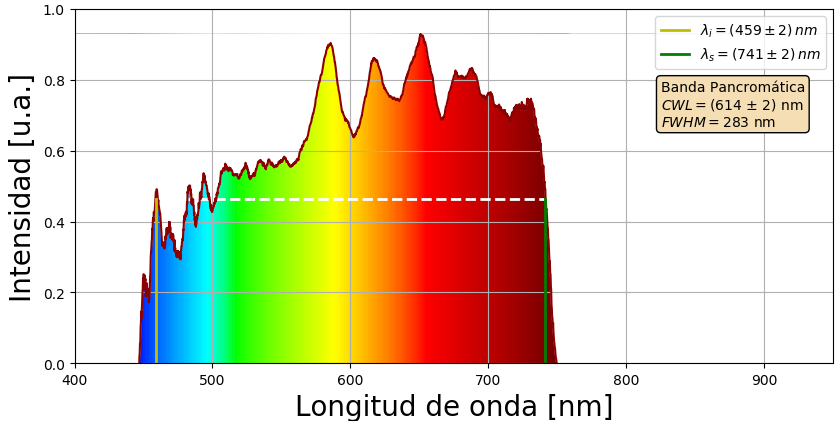
\includegraphics[width=1.0\textwidth]{Figs/microespectrometro/espectro_pancromatica.png}
	\caption{Arreglo experimental del prototipo 0.}
	\label{fig:setup0}
\end{figure}

roja
\begin{figure}[H]
	\centering
	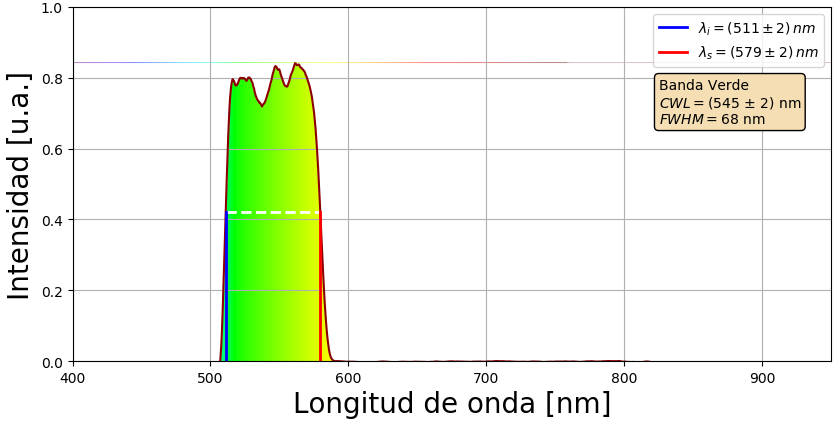
\includegraphics[width=1.0\textwidth]{Figs/microespectrometro/espectro_verde.png}
	\caption{Arreglo experimental del prototipo 0.}
	\label{fig:setup0}
\end{figure}

NIR
\begin{figure}[H]
	\centering
	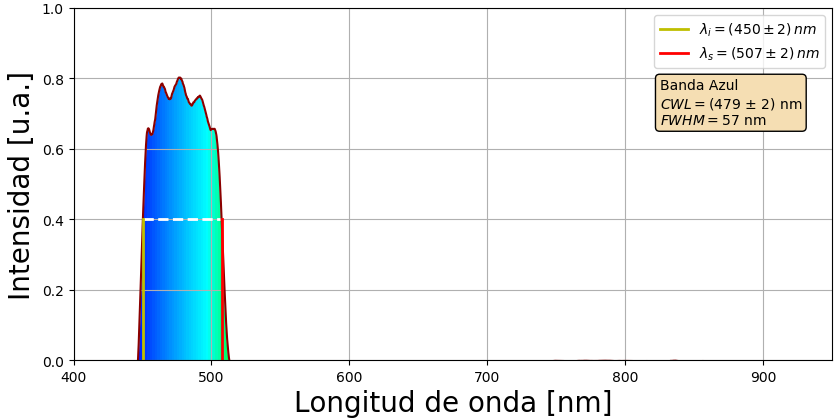
\includegraphics[width=1.0\textwidth]{Figs/microespectrometro/espectro_azul.png}
	\caption{Arreglo experimental del prototipo 0.}
	\label{fig:setup0}
\end{figure}

%%%%%%%%%%%%%%%%%%%%%%%%%%%%%%%%%%%%%%%%%%%%%%%%%%%%%%%%%%%%%%%%%%%%%%%%%%%%%%%%%%%%%%%%%%%%%%%%%%%%%%%%%%%%%%%%%%%%%%%%%%%%%%%%%%%%%%%%%%%%%%%%%%%%%%%%%%%%%%%%%%%%%%%%%%%%%%%%%%%%%%%%%%%%%%%%%%%%%%%%%%%%%%%%%%%%%%%%%%%%

\singlespacing
\subsection{Caracterización espectral de las manchas ó defectos de transmisión}
\label{sec:defctma}
\spacing{1.5}

%%%%%%%%%%%%%%%%%%%%%%%%%%%%%%%%%%%%%%%%%%%%%%%%%%%%%%%%%%%%%%%%%%%%%%%%%%%%%%%%%%%%%%%%%%%%%%%%%%%%%%%%%%%%%%%%%%%%%%%%%%%%%%%%%%%%%%%%%%%%%%%%%%%%%%%%%%%%%%%%%%%%%%%%%%%%%%%%%%%%%%%%%%%%%%%%%%%%%%%%%%%%%%%%%%%%%%%%%%%%

\singlespacing
\subsection{Caracterización espectral de los agujeros ó huecos}
\label{sec:defctag}
\spacing{1.5}
